\chapter{Arhitektura i dizajn sustava}
		
	Arhitektura se može podijeliti na tri podsustava: 
	\begin{itemize}
		\item Web poslužitelj 
		\item Web aplikacija 
		\item Baza podataka 
	\end{itemize}
	Web preglednik je program koji korisniku omogućuje pregled web stranica i multimedijalnih sadržaja vezanih uz njih. Svaki internetski preglednik je prevoditelj. Dakle, stranica je pisana u kodu koji preglednik nakon toga interpretira kako nešto svakome razumljivo. Korisnik putem web preglednika šalje zahtjev web poslužitelju. 
	
	Web poslužitelj osnova je rada web aplikacije. Njegova primarna zadaća je komunikacija klijenta s aplikacijom. Komunikacija se odvija preko HTTP (engl. Hyper Text Transfer Protocol) protokola, što je protokol u prijenosu informacija na webu. Poslužitelj je onaj koji pokreće web aplikaciju te joj prosljeđuje zahtjev. 
	
	Korisnik koristi web aplikaciju za obrađivanje željenih zahtjeva. Web aplikacija obrađuje zahtjev te ovisno o zahtjevu, pristupa bazi podataka nakon čega preko poslužitelja vraća korisniku odgovor u obliku HTML dokumenta vidljivog u web pregledniku. 
	
	Programski jezik kojeg smo odabrali za izradu naše web aplikacije je Java Spring Boot. Odabrano razvojno okruženje je Eclipse IDE. Arhitektura sustava temeljiti će se na MVC (Model-View-Controller) konceptu. 
	
	Karakteristika MVC koncepta je nezavisan razvoj pojedinih dijelova aplikacije što za posljedicu ima jednostavnije ispitivanje kao i jednostavnije razvijanje i dodavanje novih svojstava u sustav. \\
	
	MVC koncept sastoji se od: 
	\begin{itemize}
		\item Model - Središnja komponenta sustava. Predstavlja dinamičke strukture podataka, neovisne o korisničkom sučelju. Izravno upravlja podacima, logikom i pravilima aplikacije. Također prima ulazne podatke od Controllera 
		\item View - Bilo kakav prikaz podataka, poput grafa. Mogući su različiti prikazi iste informacije poput grafičkog ili tabličnog prikaza podatak. 
		\item Controller – Prima ulaze i prilagođava ih za prosljeđivanje Model-u ili View-u. Upravlja korisničkim zahtjevima i na temelju njih izvodi daljnju interakciju s ostalim elementima sustava. 
	\end{itemize}
		

		

				
		\section{Baza podataka}
			
			\textbf{\textit{dio 1. revizije}}\\
			
		%\textit{Potrebno je opisati koju vrstu i implementaciju baze podataka ste odabrali, glavne komponente od kojih se sastoji i slično.}
		Baza podataka je predstavljena pomoću ER te relacijskog dijagrama. Od glavnih komponenti, primarno se pojavljuju:
		\begin{itemize}
		\item Employee
		\item Role
		\item Group
		\item EmployeeGroup
		\item Job
		\item Task
		\item EmployeeTask
		\item Location
		\item WorkHoursInput
	    \end{itemize}
		
			\subsection{Opis tablica}
			

				%\textit{Svaku tablicu je potrebno opisati po zadanom predlošku. Lijevo se nalazi točno ime varijable u bazi podataka, u sredini se nalazi tip podataka, a desno se nalazi opis varijable. Svjetlozelenom bojom označite primarni ključ. Svjetlo plavom označite strani ključ}
				
				\subsubsection{Employee}
					Sadrži podatke o djelatniku, uključujući osobne podatke i podatke za prijavu (korisničko ime i lozinka).
				
					\begin{longtabu} to \textwidth {|X[6, l]|X[6, l]|X[20, l]|}
						
						\hline \multicolumn{3}{|c|}{\textbf{Employee}}	 \\[3pt] \hline
						\endfirsthead
						
						\hline \multicolumn{3}{|c|}{\textbf{Employee}}	 \\[3pt] \hline
						\endhead
						
						\hline 
						\endlastfoot

						\cellcolor{LightGreen}pid & CHAR & Osobni identifikacijski broj djelatnika.		\\ \hline
						name	& VARCHAR & Ime djelatnika.  	\\ \hline 
						surname & VARCHAR & Prezime djelatnika.  \\ \hline 
						email & VARCHAR & E-mail adresa.		\\ \hline
						username & VARCHAR	& Jedinstveno korisničko ime djelatnika.	\\ \hline
						password & VARCHAR & Lozinka djelatnika.		\\ \hline   
						\cellcolor{LightBlue} idRole & INTEGER & Identifikator uloge djelatnika. 	\\ \hline 
						
						
					\end{longtabu}

				\subsubsection{Role}
					Sadrži podatke o ulozi korisnika. Uloga može biti: direktor, vođa tima ili djelatnik.
					
					\begin{longtabu} to \textwidth {|X[6, l]|X[6, l]|X[20, l]|}
						
						\hline \multicolumn{3}{|c|}{\textbf{Role}}	 \\[3pt] \hline
						\endfirsthead
						
						\hline \multicolumn{3}{|c|}{\textbf{Role}}	 \\[3pt] \hline
						\endhead
						
						\hline 
						\endlastfoot
						
						\cellcolor{LightGreen}idRole & INTEGER	& Identifikator uloge.	\\ \hline
						name & VARCHAR & Naziv uloge (direktor, vođa tima, djelatnik).  	\\ \hline 					
						
					\end{longtabu}
				
				\subsubsection{Group}
					Djelatnici rade u grupama. Grupa ima svog voditelja - djelatnika kojem je direktor dodijelio ulogu voditelja. Grupa može biti stvorena bez članova, ali ne može biti bez voditelja. Svaka se grupa bavi nekom djelatnosti. 
					
					\begin{longtabu} to \textwidth {|X[6, l]|X[6, l]|X[20, l]|}
						
						\hline \multicolumn{3}{|c|}{\textbf{Group}}	 \\[3pt] \hline
						\endfirsthead
						
						\hline \multicolumn{3}{|c|}{\textbf{Group}}	 \\[3pt] \hline
						\endhead
						
						\hline 
						\endlastfoot
						
						\cellcolor{Lightgreen} idGroup & INTEGER	& Identifikator grupe.	\\ \hline
						name	& VARCHAR & Naziv grupe.  	\\ \hline    
						\cellcolor{LightBlue} idLeader & INTEGER & Identifikator voditelja grupe. 	\\ \hline 
						\cellcolor{LightBlue} idJob & INTEGER & Identifikator djelatnosti kojom se grupa bavi. 	\\ \hline 
						
					\end{longtabu}
			
				\subsubsection{EmployeeGroup}
					Tablica koja ostvaruje vezu više-na-više između tablica Employee i Group, tj. asocira djelatnike s grupama čiji su članovi. Djelatnik može istovremeno raditi u više grupa.
					
					\begin{longtabu} to \textwidth {|X[6, l]|X[6, l]|X[20, l]|}
						
						\hline \multicolumn{3}{|c|}{\textbf{EmployeeGroup}}	 \\[3pt] \hline
						\endfirsthead
						
						\hline \multicolumn{3}{|c|}{\textbf{EmployeeGroup}}	 \\[3pt] \hline
						\endhead
						
						\hline 
						\endlastfoot
						
						\cellcolor{LightGreen}idEmployee & CHAR	& Identifikator djelatnika.	\\ \hline
						\cellcolor{LightGreen}idGroup & INTEGER	& Identifikator grupe.	\\ \hline
						
					\end{longtabu}
				
				\subsubsection{Job}
					Sadrži podatke o djelatnosti kojima se tvrtka bavi. Svakoj djelatnosti pridružen je naziv i tekstualni opis.
					
					\begin{longtabu} to \textwidth {|X[6, l]|X[6, l]|X[20, l]|}
						
						\hline \multicolumn{3}{|c|}{\textbf{Job}}	 \\[3pt] \hline
						\endfirsthead
						
						\hline \multicolumn{3}{|c|}{\textbf{Job}}	 \\[3pt] \hline
						\endhead
						
						\hline 
						\endlastfoot
						
						\cellcolor{LightGreen}idJob & INTEGER	& Identifikator djelatnosti.	\\ \hline
						name & VARCHAR	& Naziv djelatnosti.	\\ \hline
						description & TEXT	& Opis djelatnosti.	\\ \hline
						
					\end{longtabu}
				
				\subsubsection{Task}
					Zadaci na kojima djelatnici rade, a zadaje ih voditelj grupe za djelatnike kojima je nadležan. Svaki zadatak ima naziv i opis, datum i vrijeme planiranog početka i završetka, te procjenu broja radnih sati koji će biti potrebni da bi se zadatak dovršio. Voditelj grupe može i pridružiti zadatak nekoj djelatnosti. Zadatak se može obavljati na nekoj lokaciji. Pri stvaranju zadatka, voditelj određuje planirani trošak i prihod. Kada djelatnik dovrši zadatak, stvarni trošak i prihod se upisuju u tablicu.
					
					\begin{longtabu} to \textwidth {|X[10, l]|X[6, l]|X[16, l]|}
						
						\hline \multicolumn{3}{|c|}{\textbf{Task}}	 \\[3pt] \hline
						\endfirsthead
						
						\hline \multicolumn{3}{|c|}{\textbf{Task}}	 \\[3pt] \hline
						\endhead
						
						\hline 
						\endlastfoot
						
						\cellcolor{LightGreen}idTask & INTEGER	& Identifikator zadatka.	\\ \hline
						name & VARCHAR	& Naziv zadatka.	\\ \hline
						description & TEXT	& Tekstualni opis zadatka.	\\ \hline
						dateTimeStart & TIMESTAMP	& Datum i vrijeme početka zadatka. Mora biti manje vrijednosti od polja datumVrijemeZavrsetka.	\\ \hline
						dateTimeEnd & TIMESTAMP	& Datum i vrijeme završetka zadatka. Mora biti veće vrijednosti od polja datumVrijemePocetka.	\\ \hline
						hoursNeededEstimate & SMALLINT	& Procjena broja radnih sati potrebnih za dovršetak zadatka. Procjenu određuje voditelj tima koji je zadao zadatak. Procjena može, ali ne mora odgovarati razlici između dateTimeEnd i dateTimeStart. \\ \hline
						plannedCost & FLOAT & Planirani trošak. \\ \hline
						realizedCost & FLOAT & Realizirani trošak. \\ \hline
						plannedProfit & FLOAT & Planirana dobit. \\ \hline
						realizedProfit & FLOAT & Realizirana dobit. \\ \hline
						\cellcolor{LightBlue}idJob & INTEGER	& Identifikator djelatnosti kojoj zadatak pripada.	\\ \hline
						\cellcolor{LightBlue}idLocation & INTEGER	& Identifikator lokacije na kojoj se zadatak obavlja.	\\ \hline
						
					\end{longtabu}
				
				\subsubsection{EmployeeTask}
					Tablica koja ostvaruje vezu više-na-više između tablica Employee i Task, tj. određuje koji djelatnik radi na kojim zadacima. Zapisuje se i realizacija zadatka koja predstavlja postotak dovršenog posla. Na početku iznosi 0 i povećava se kako djelatnik napreduje s poslom.
					
					\begin{longtabu} to \textwidth {|X[6, l]|X[6, l]|X[20, l]|}
						
						\hline \multicolumn{3}{|c|}{\textbf{EmployeeTask}}	 \\[3pt] \hline
						\endfirsthead
						
						\hline \multicolumn{3}{|c|}{\textbf{EmployeeTask}}	 \\[3pt] \hline
						\endhead
						
						\hline 
						\endlastfoot
						
						\cellcolor{LightGreen}idEmployee & CHAR	& Identifikator djelatnika koji radi na zadatku.	\\ \hline
						\cellcolor{LightGreen}idTask & INTEGER	& Identifikator zadatka na kojem djelatnik radi.	\\ \hline
						realized & SMALLINT & Postotak posla kojeg je djelatnik obavio na zadatku u odnosu na ukupan posao. Može biti u intervalu [0, 100]. Početna vrijednost je 0. \\ \hline
						
					\end{longtabu}
			
				\subsubsection{Location}
					Lokacije na kojima se obavljaju poslovi. Za svaku lokaciju zapisuje se adresa, mjesto i geografska širina i dužina radi prikaza na karti.
					
					\begin{longtabu} to \textwidth {|X[6, l]|X[6, l]|X[20, l]|}
						
						\hline \multicolumn{3}{|c|}{\textbf{Location}}	 \\[3pt] \hline
						\endfirsthead
						
						\hline \multicolumn{3}{|c|}{\textbf{Location}}	 \\[3pt] \hline
						\endhead
						
						\hline 
						\endlastfoot
						
						\cellcolor{LightGreen}idLocation & INTEGER	& Identifikator lokacije.	\\ \hline
						address & VARCHAR & Adresa na kojoj se lokacija nalazi. \\ \hline
						placeName & VARCHAR & Mjesto u kojem se lokacija nalazi. \\ \hline
						latitude & DOUBLE & Geografska širina lokacije. \\ \hline
						longitude & DOUBLE & Geografska dužina lokacije. \\ \hline
						
					\end{longtabu}
				
				\subsubsection{WorkHoursInput}
					Tablica koja predstavlja evidenciju radnih sati djelatnika. Svaki djelatnik upisuje koliko je sati odradio na kojem zadatku svaki radni dan.
					 
					\begin{longtabu} to \textwidth {|X[8, l]|X[6, l]|X[18, l]|}
						
						\hline \multicolumn{3}{|c|}{\textbf{WorkHoursInput}}	 \\[3pt] \hline
						\endfirsthead
						
						\hline \multicolumn{3}{|c|}{\textbf{WorkHoursInput}}	 \\[3pt] \hline
						\endhead
						
						\hline 
						\endlastfoot
						
						\cellcolor{LightGreen}idWorkHoursInput & INTEGER	& Identifikator unosa.	\\ \hline
						date & DATE & Datum unosa. \\ \hline
						workHoursDone & SMALLINT & Broj radnih sati koje je djelatnik odradio na zadatku tog dana. \\ \hline
						\cellcolor{LightBlue}idEmployee & CHAR & Identifikator djelatnika koji obavlja unos. \\ \hline
						\cellcolor{LightBlue}idTask & INTEGER & Identifikator zadatka na kojeg se unos odnosi. \\
						
					\end{longtabu}
						
			\subsection{Dijagram baze podataka}
				%\textit{ U ovom potpoglavlju potrebno je umetnuti dijagram baze podataka. Primarni i strani ključevi moraju biti označeni, a tablice povezane. Bazu podataka je potrebno normalizirati. Podsjetite se kolegija "Baze podataka".}
				
				\begin{figure}[H]
					\centering
					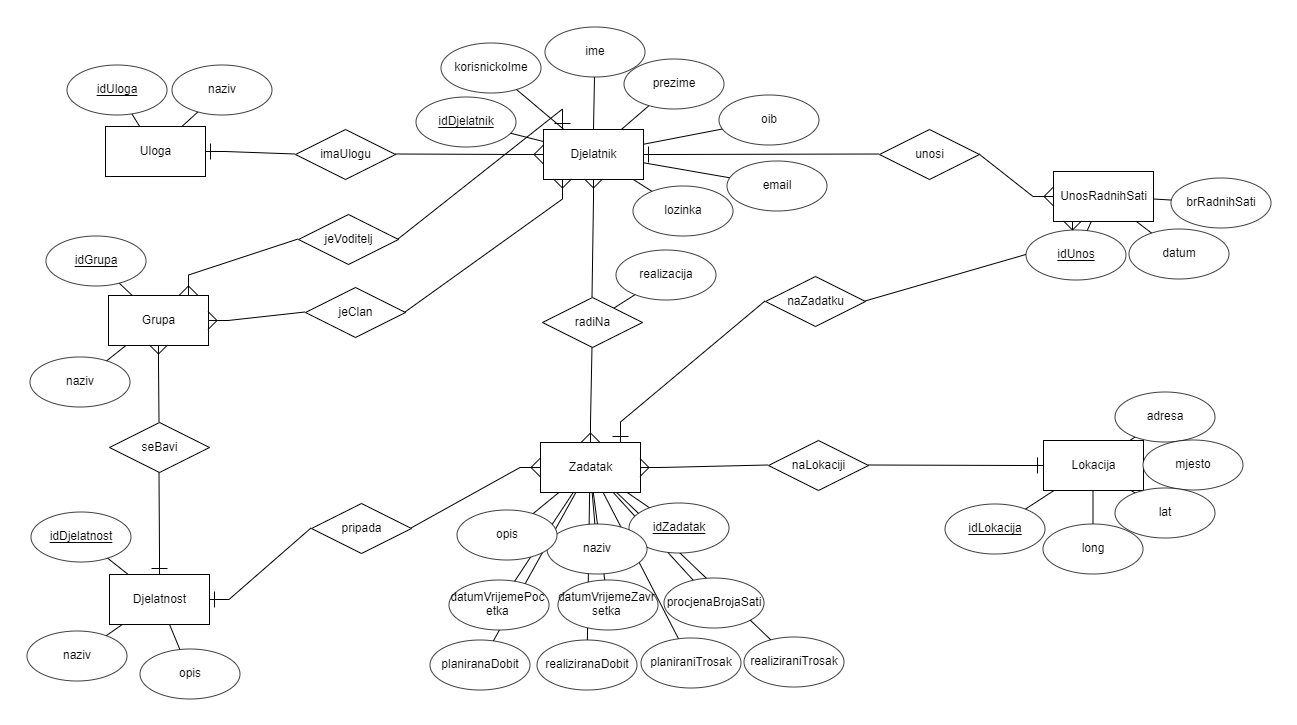
\includegraphics[width=\textwidth]{slike/ERdijagram.png}
					\caption{ER dijagram baze podataka}
				\end{figure}
			
				\begin{figure}[H]
					\centering
					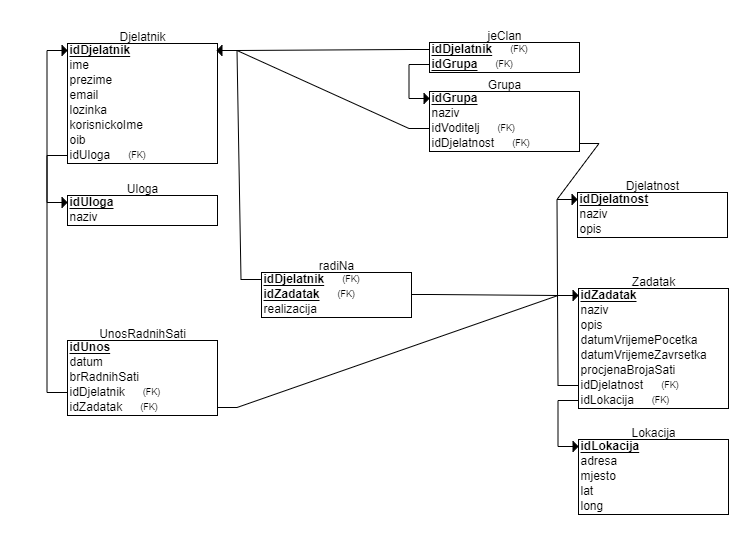
\includegraphics[width=\textwidth]{slike/RelDijagram.png}
					\caption{Relacijski dijagram baze podataka}
				\end{figure}		
			\eject
			
			
		\section{Dijagram razreda}
		
			%\textit{Potrebno je priložiti dijagram razreda s pripadajućim opisom. Zbog preglednosti je moguće dijagram razlomiti na više njih, ali moraju biti grupirani prema sličnim razinama apstrakcije i srodnim funkcionalnostima.}\\
			
			%\textbf{\textit{dio 1. revizije}}\\
			
			%\textit{Prilikom prve predaje projekta, potrebno je priložiti potpuno razrađen dijagram razreda vezan uz \textbf{generičku funkcionalnost} sustava. Ostale funkcionalnosti trebaju biti idejno razrađene u dijagramu sa sljedećim komponentama: nazivi razreda, nazivi metoda i vrste pristupa metodama (npr. javni, zaštićeni), nazivi atributa razreda, veze i odnosi između razreda.}\\
			
			%\textbf{\textit{dio 2. revizije}}\\			
			
			%\textit{Prilikom druge predaje projekta dijagram razreda i opisi moraju odgovarati stvarnom stanju implementacije}
			
			Na slikama su prikazani razredi koji pripadaju backend dijelu aplikacije. Dijagrame sačinjavaju razredi te među njima uočavamo dijelove poslužiteljskog sloja, odnosno entitete, objekte za prijenos podataka (engl. Data Transfer Object), repozitorije, servise i kontrolere.  

            Entiteti su klase koje predstavljaju tablice spremljene u bazi podataka. Svaka instanca entiteta predstavlja jedan redak u toj tablici.  

            Objekti za prijenos podataka su objekti koji se koriste za komunikaciju između poslužiteljskog i klijentskog dijela aplikacije. Korisni su jer pomoću njih prenosimo samo ono što je bitno, isključivo nužne podatke o određenim entitetima, no ne i cijele entitete. 
            
            Repozitoriji su Java sučelja koje upravljaju tokom podataka između poslužitelja i baze podataka. Klase repozitorija služe kao mehanizam za enkapsulaciju pohrane, dohvaćanja i pretraživanja podataka.  
            
            Servisi su klase koje sadrže poslovnu logiku aplikacije. U njima se nalaze metode čija je zadaća izvršavanje operacija nad bazom podataka, odnosno pozivanje metoda definiranih u repozitorijima. 
            
            Kontroleri, odnosno REST (engl. Representational State Transfer) kontroleri presreću dolazeće zahtjeve, pretvaraju podatke iz zahtjeva u unutarnju strukturu podataka, šalju podatke modelu na daljnju obradu te dobivaju određene podatke iz modela i prosljeđuju ih u klijentski dio aplikacije kako bi se prikazali korisniku.  
            
            Iz naziva i tipova atributa u razredima može se zaključiti vrsta ovisnosti među različitim razredima prikazanima na priloženim dijagramima. 
			
			
			\begin{figure}[H]
					\centering
					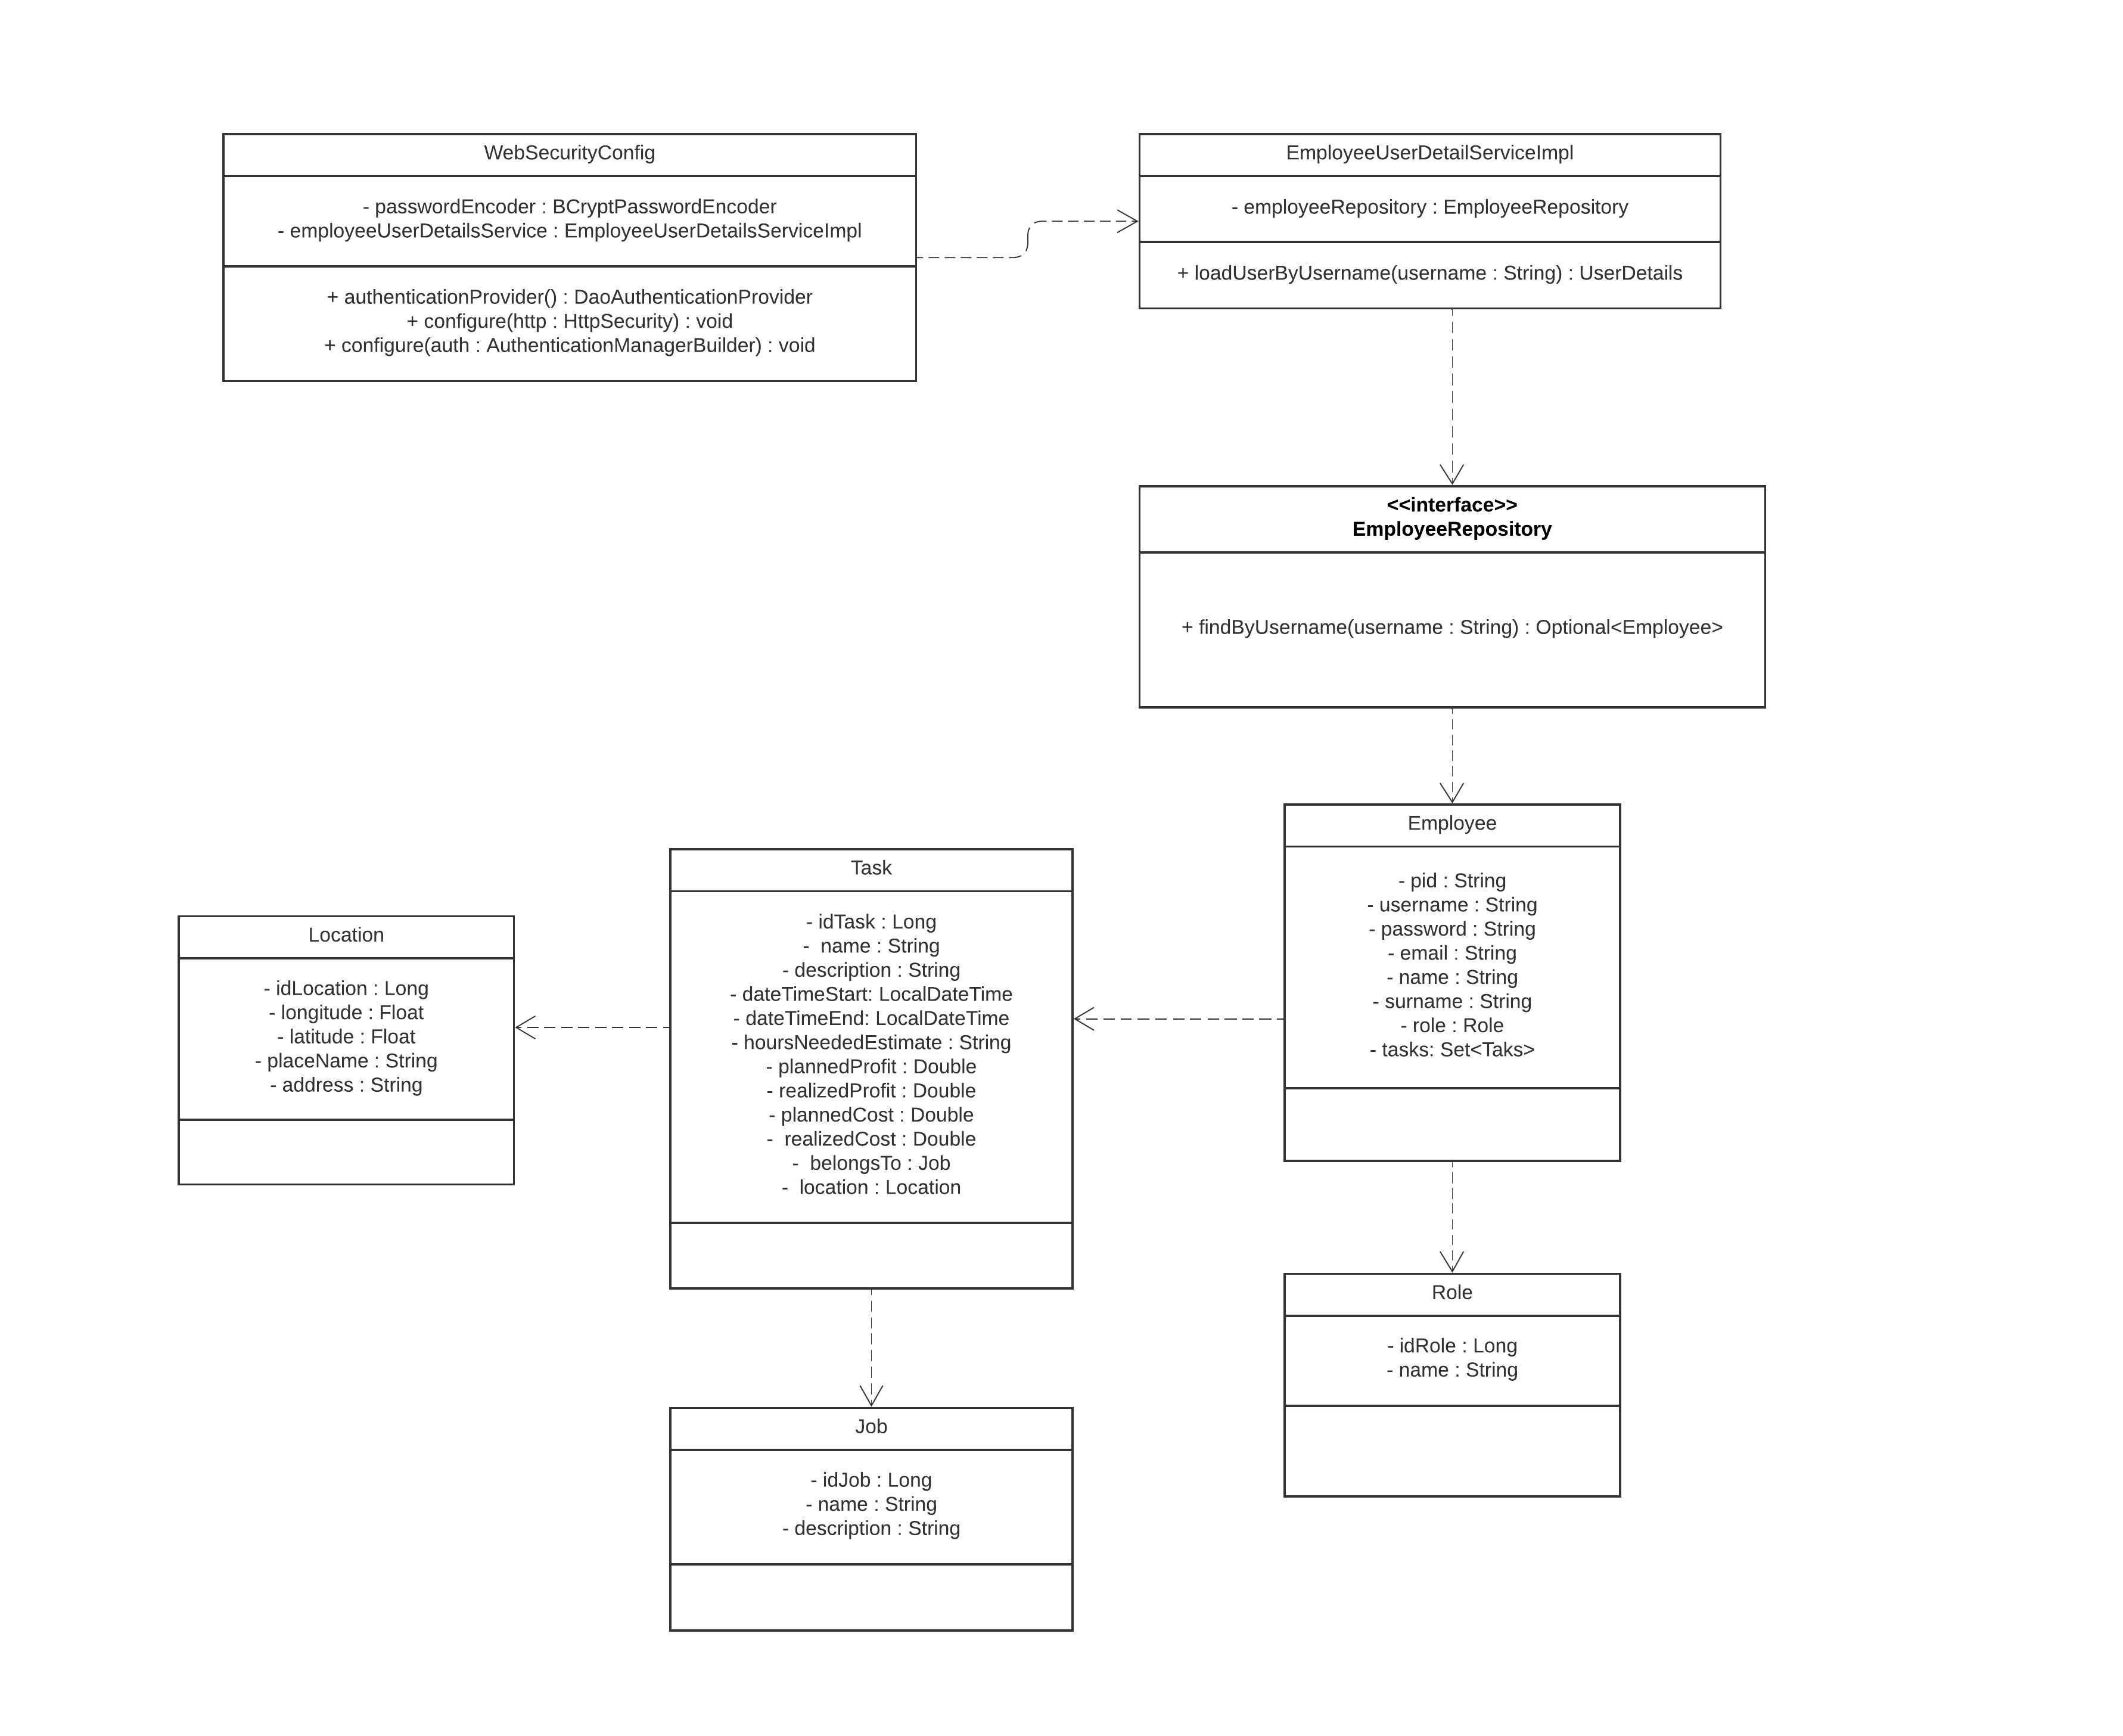
\includegraphics[width=\textwidth]{slike/Dijagram razreda - WebSecurityConfig.jpeg}
					\caption{Dijagram razreda WebSecurityConfig}
				\end{figure}
			
			
			\eject
			\begin{figure}[H]
					\centering
					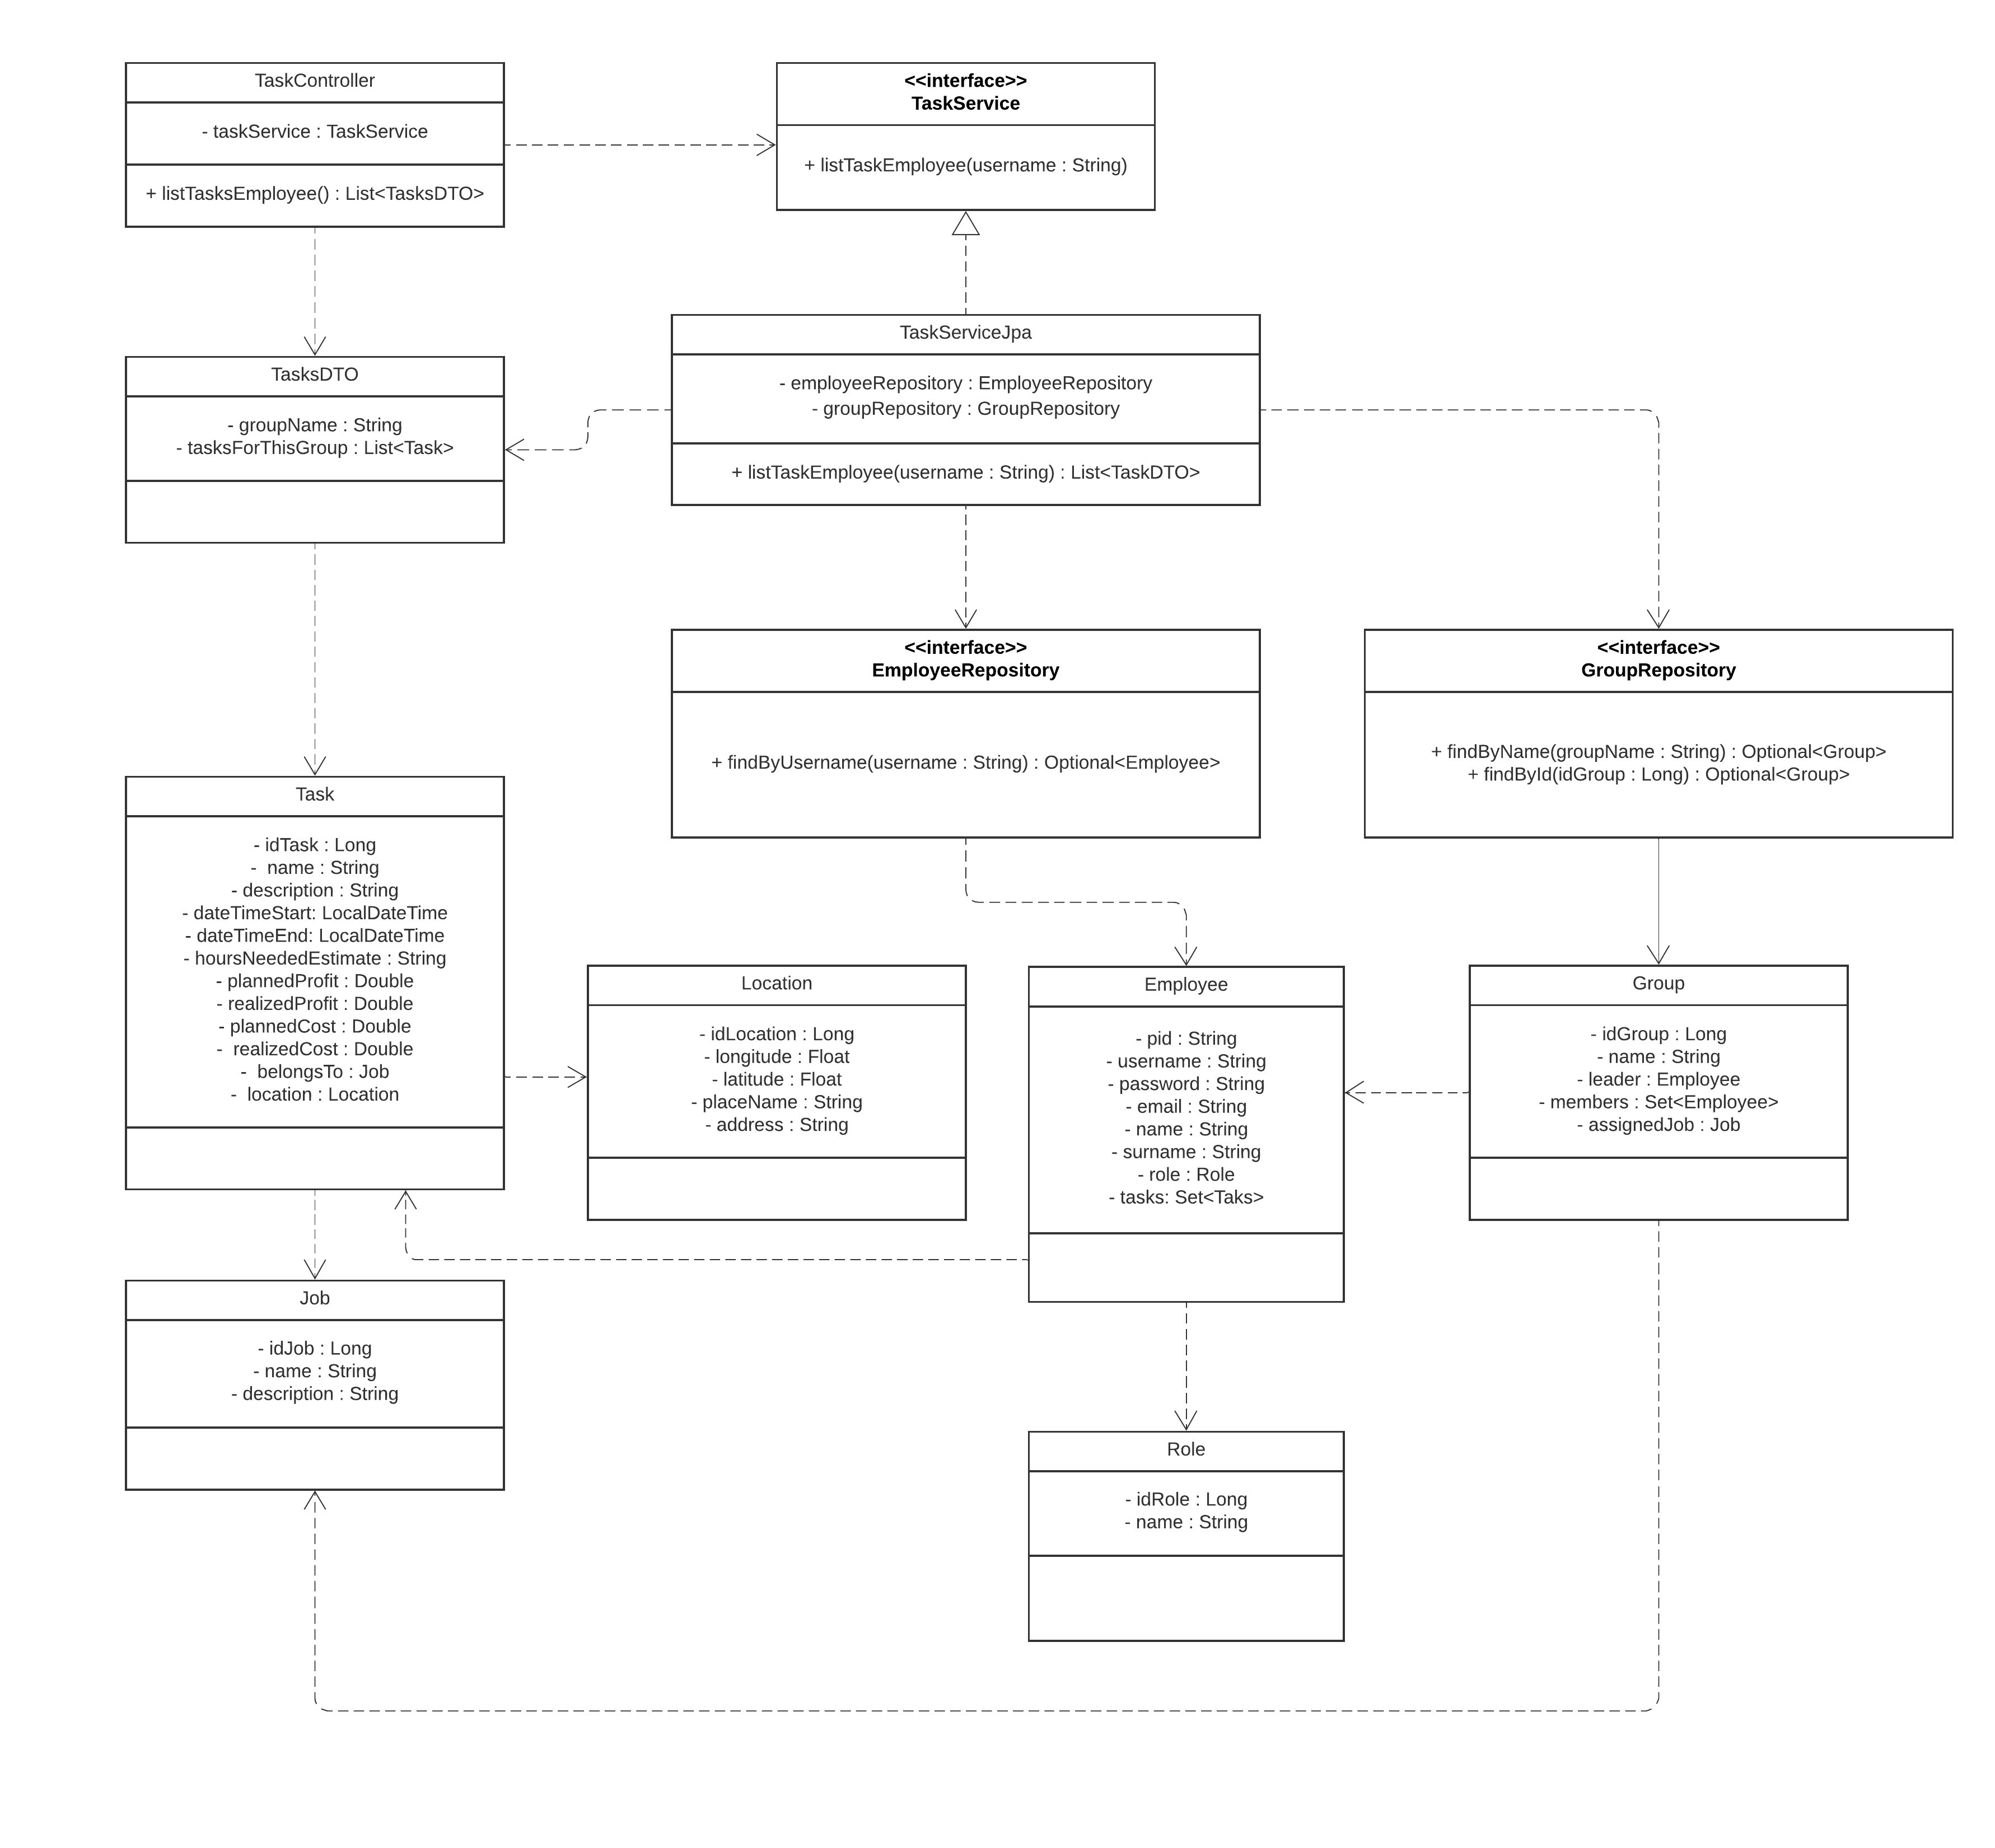
\includegraphics[width=\textwidth]{slike/Dijagram razreda - TaskController.jpg}
					\caption{Dijagram razreda TaskController}
				\end{figure}
			
			
			\eject
			\begin{figure}[H]
					\centering
					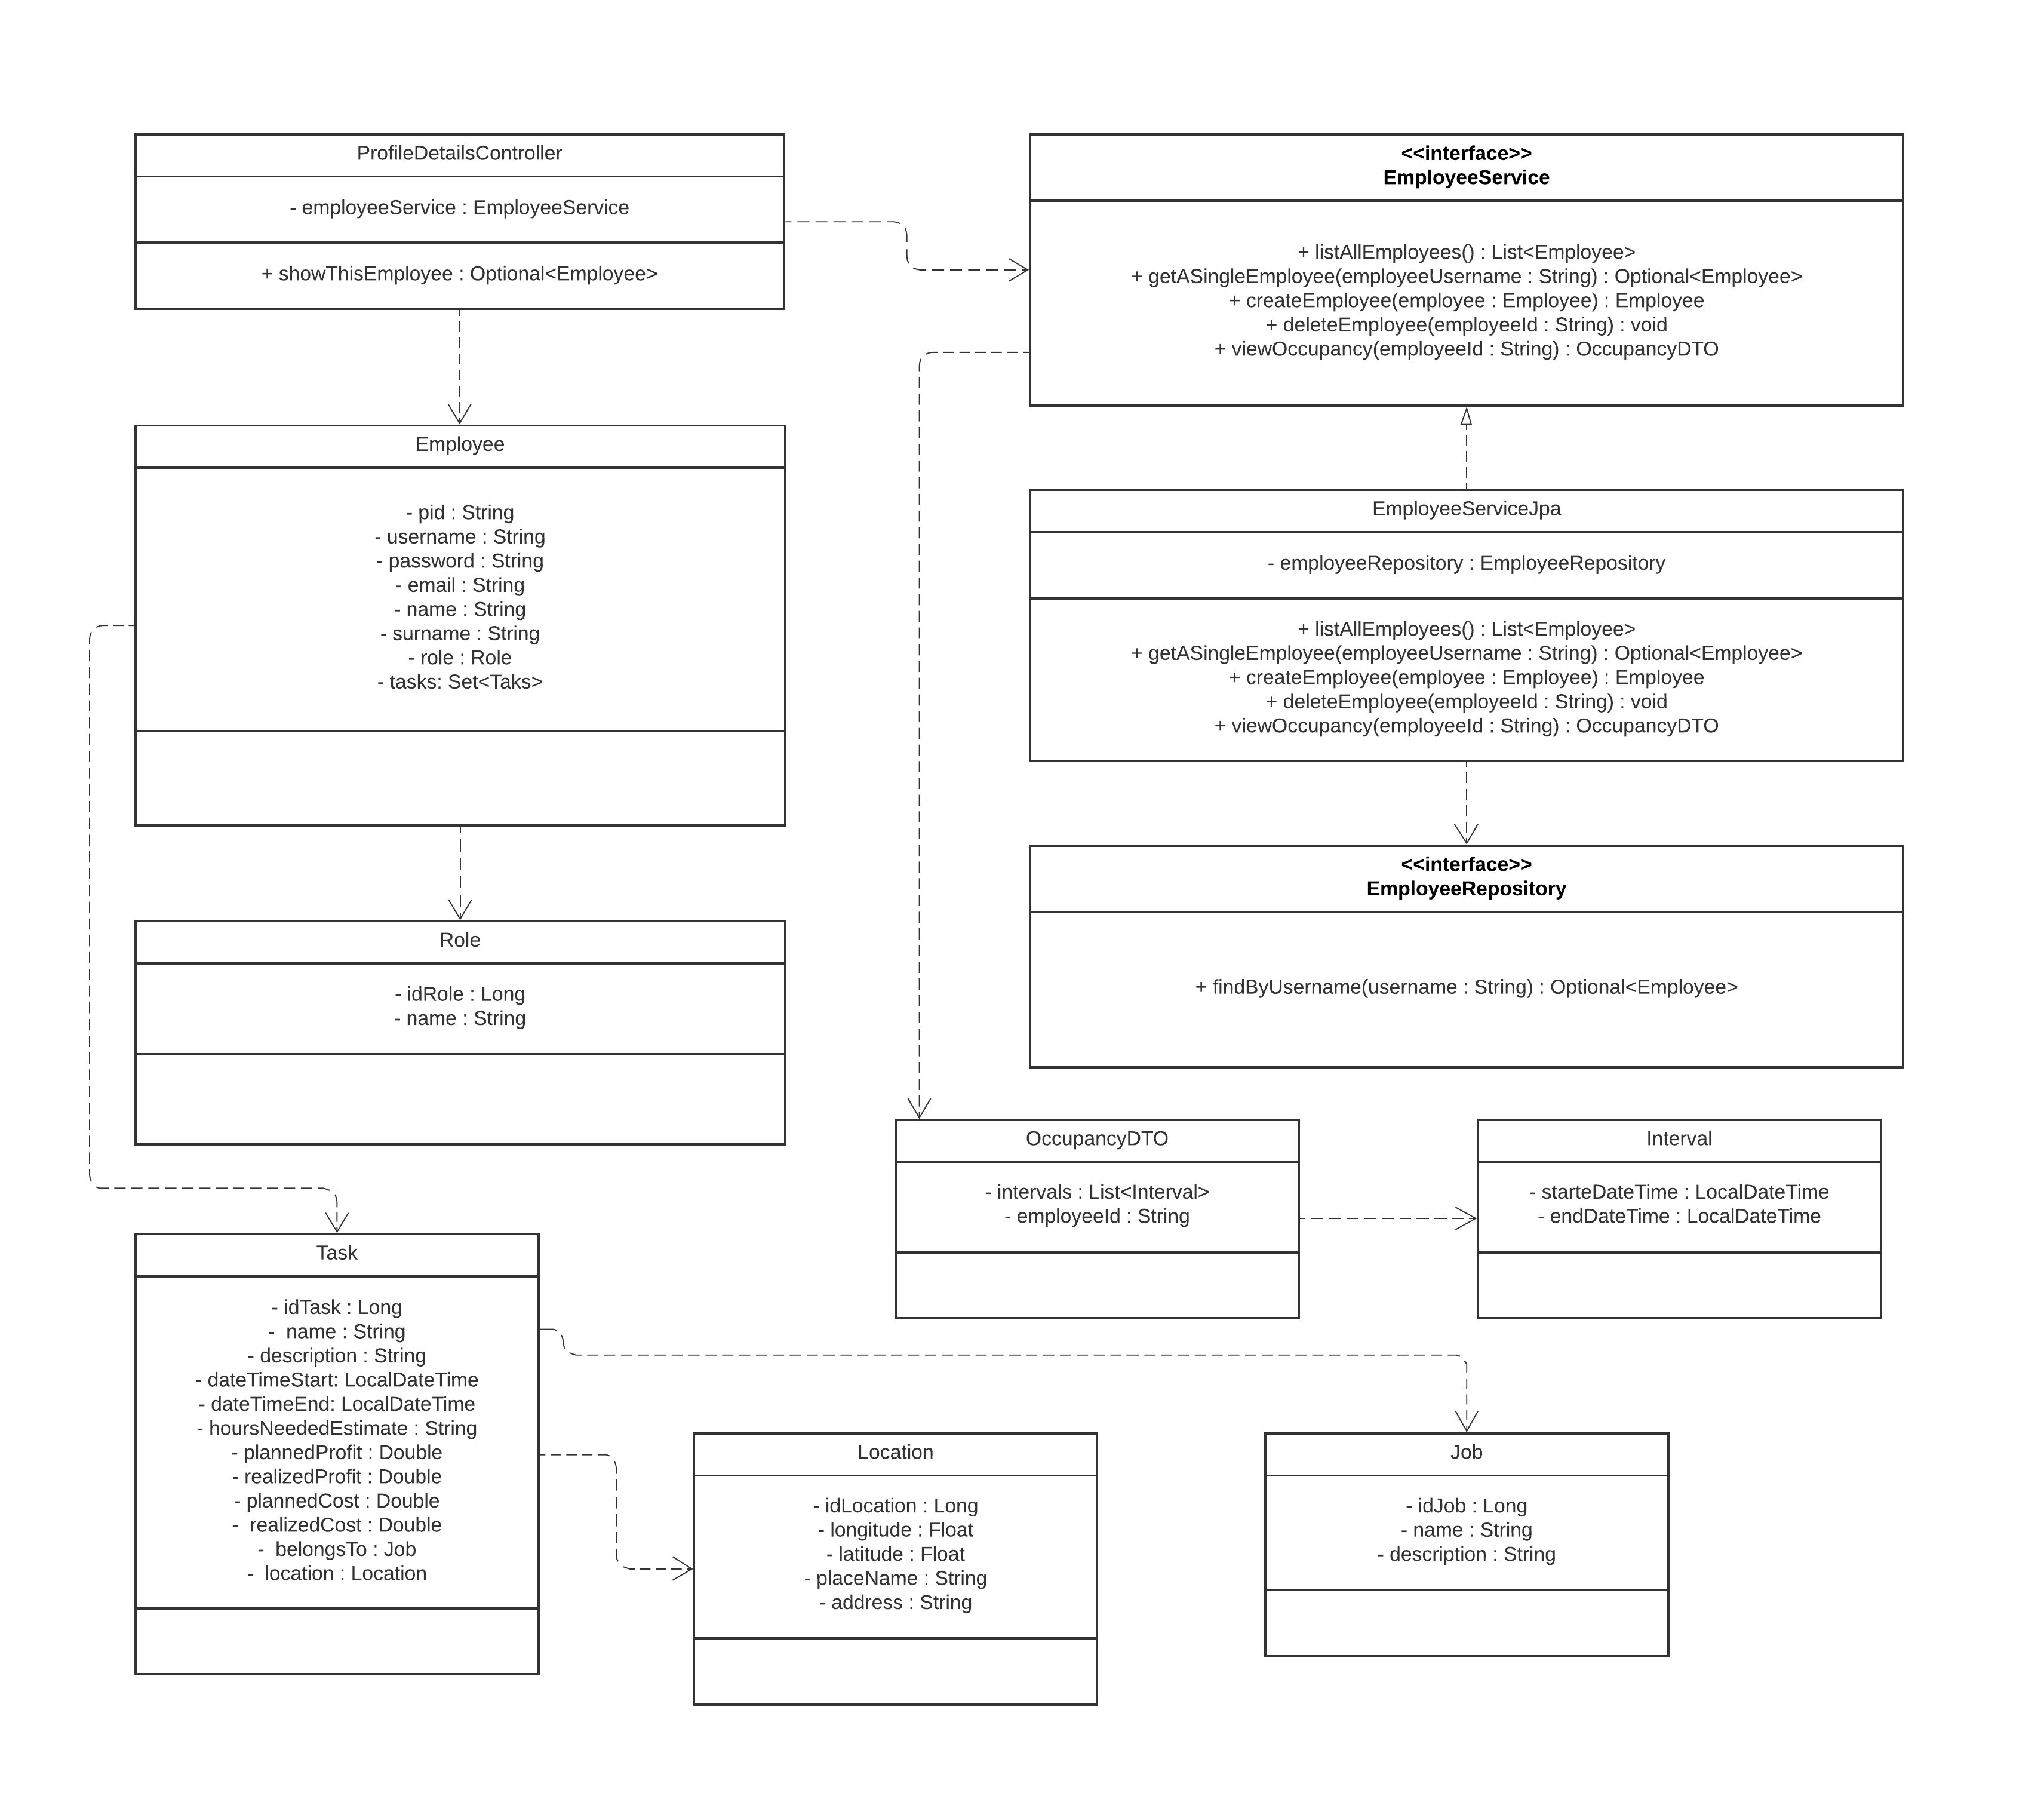
\includegraphics[width=\textwidth]{slike/Dijagram razreda - ProfileDetailsController.jpg}
					\caption{Dijagram razreda ProfileDetailsController}
				\end{figure}
			
			
			\eject
			\begin{figure}[H]
					\centering
					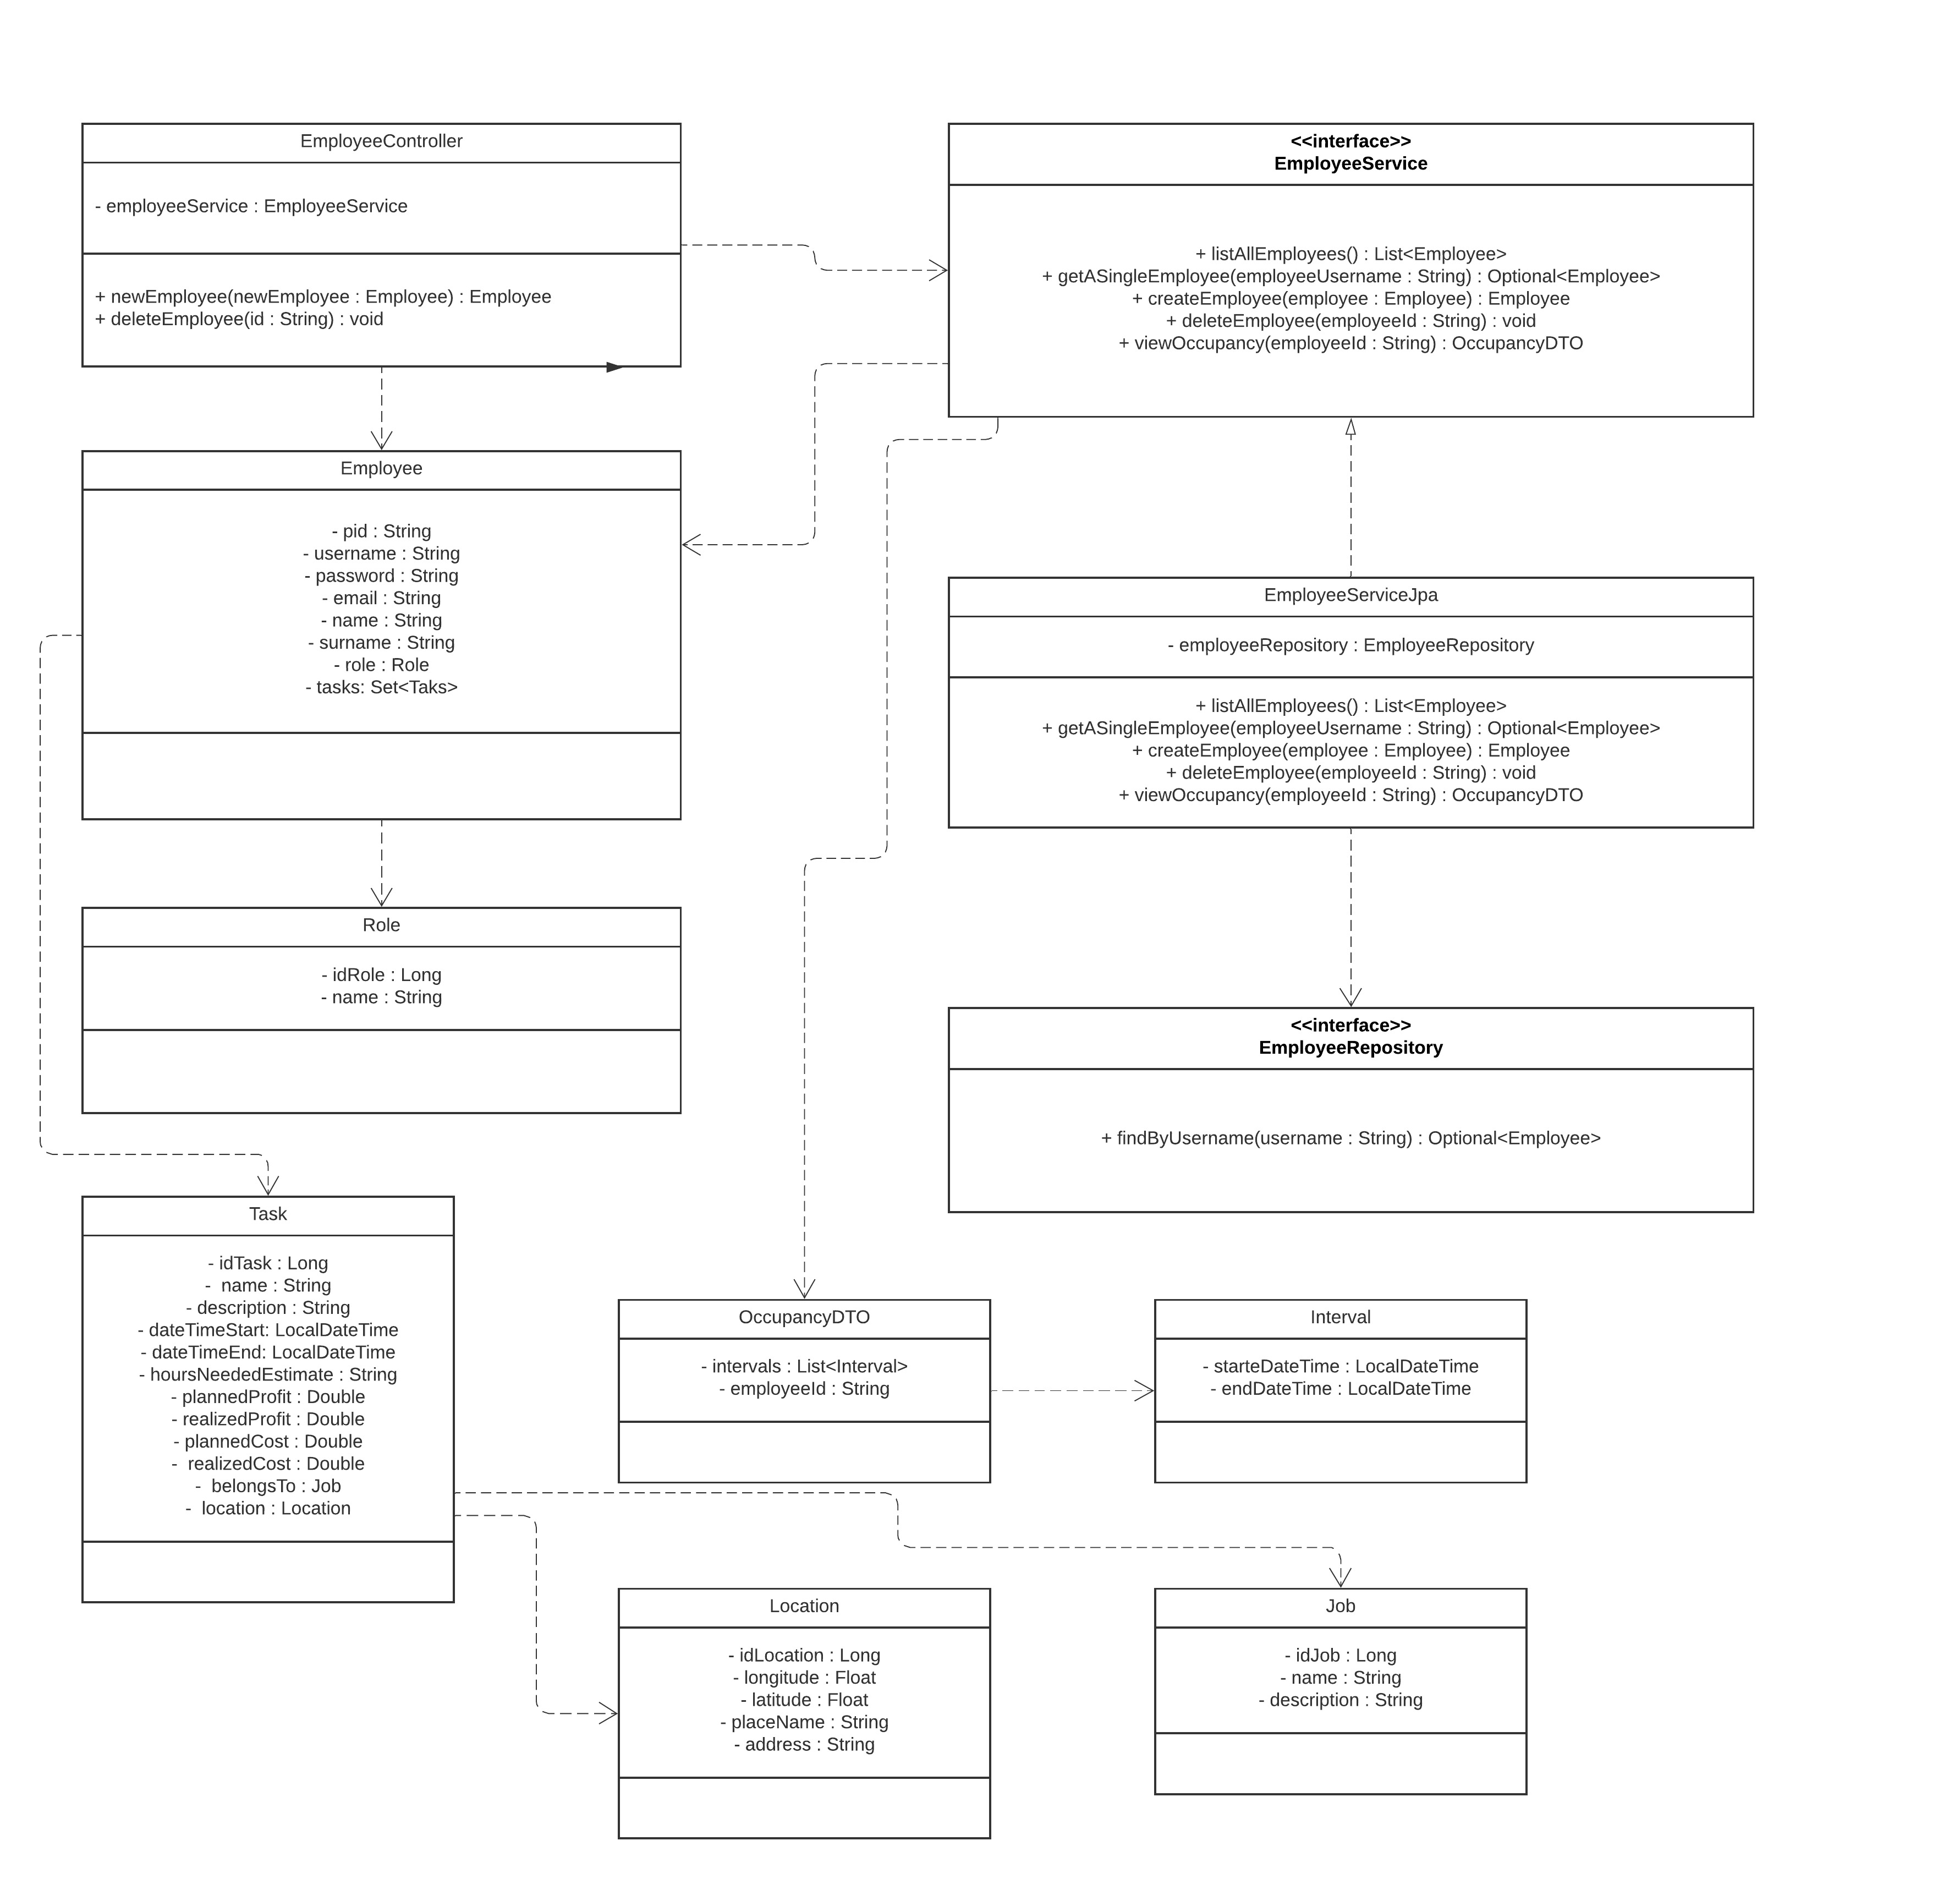
\includegraphics[width=\textwidth]{slike/Dijagram razreda - EmployeeController.jpg}
					\caption{Dijagram razreda EmployeeController}
				\end{figure}
			
			
			\eject
			\begin{figure}[H]
					\centering
					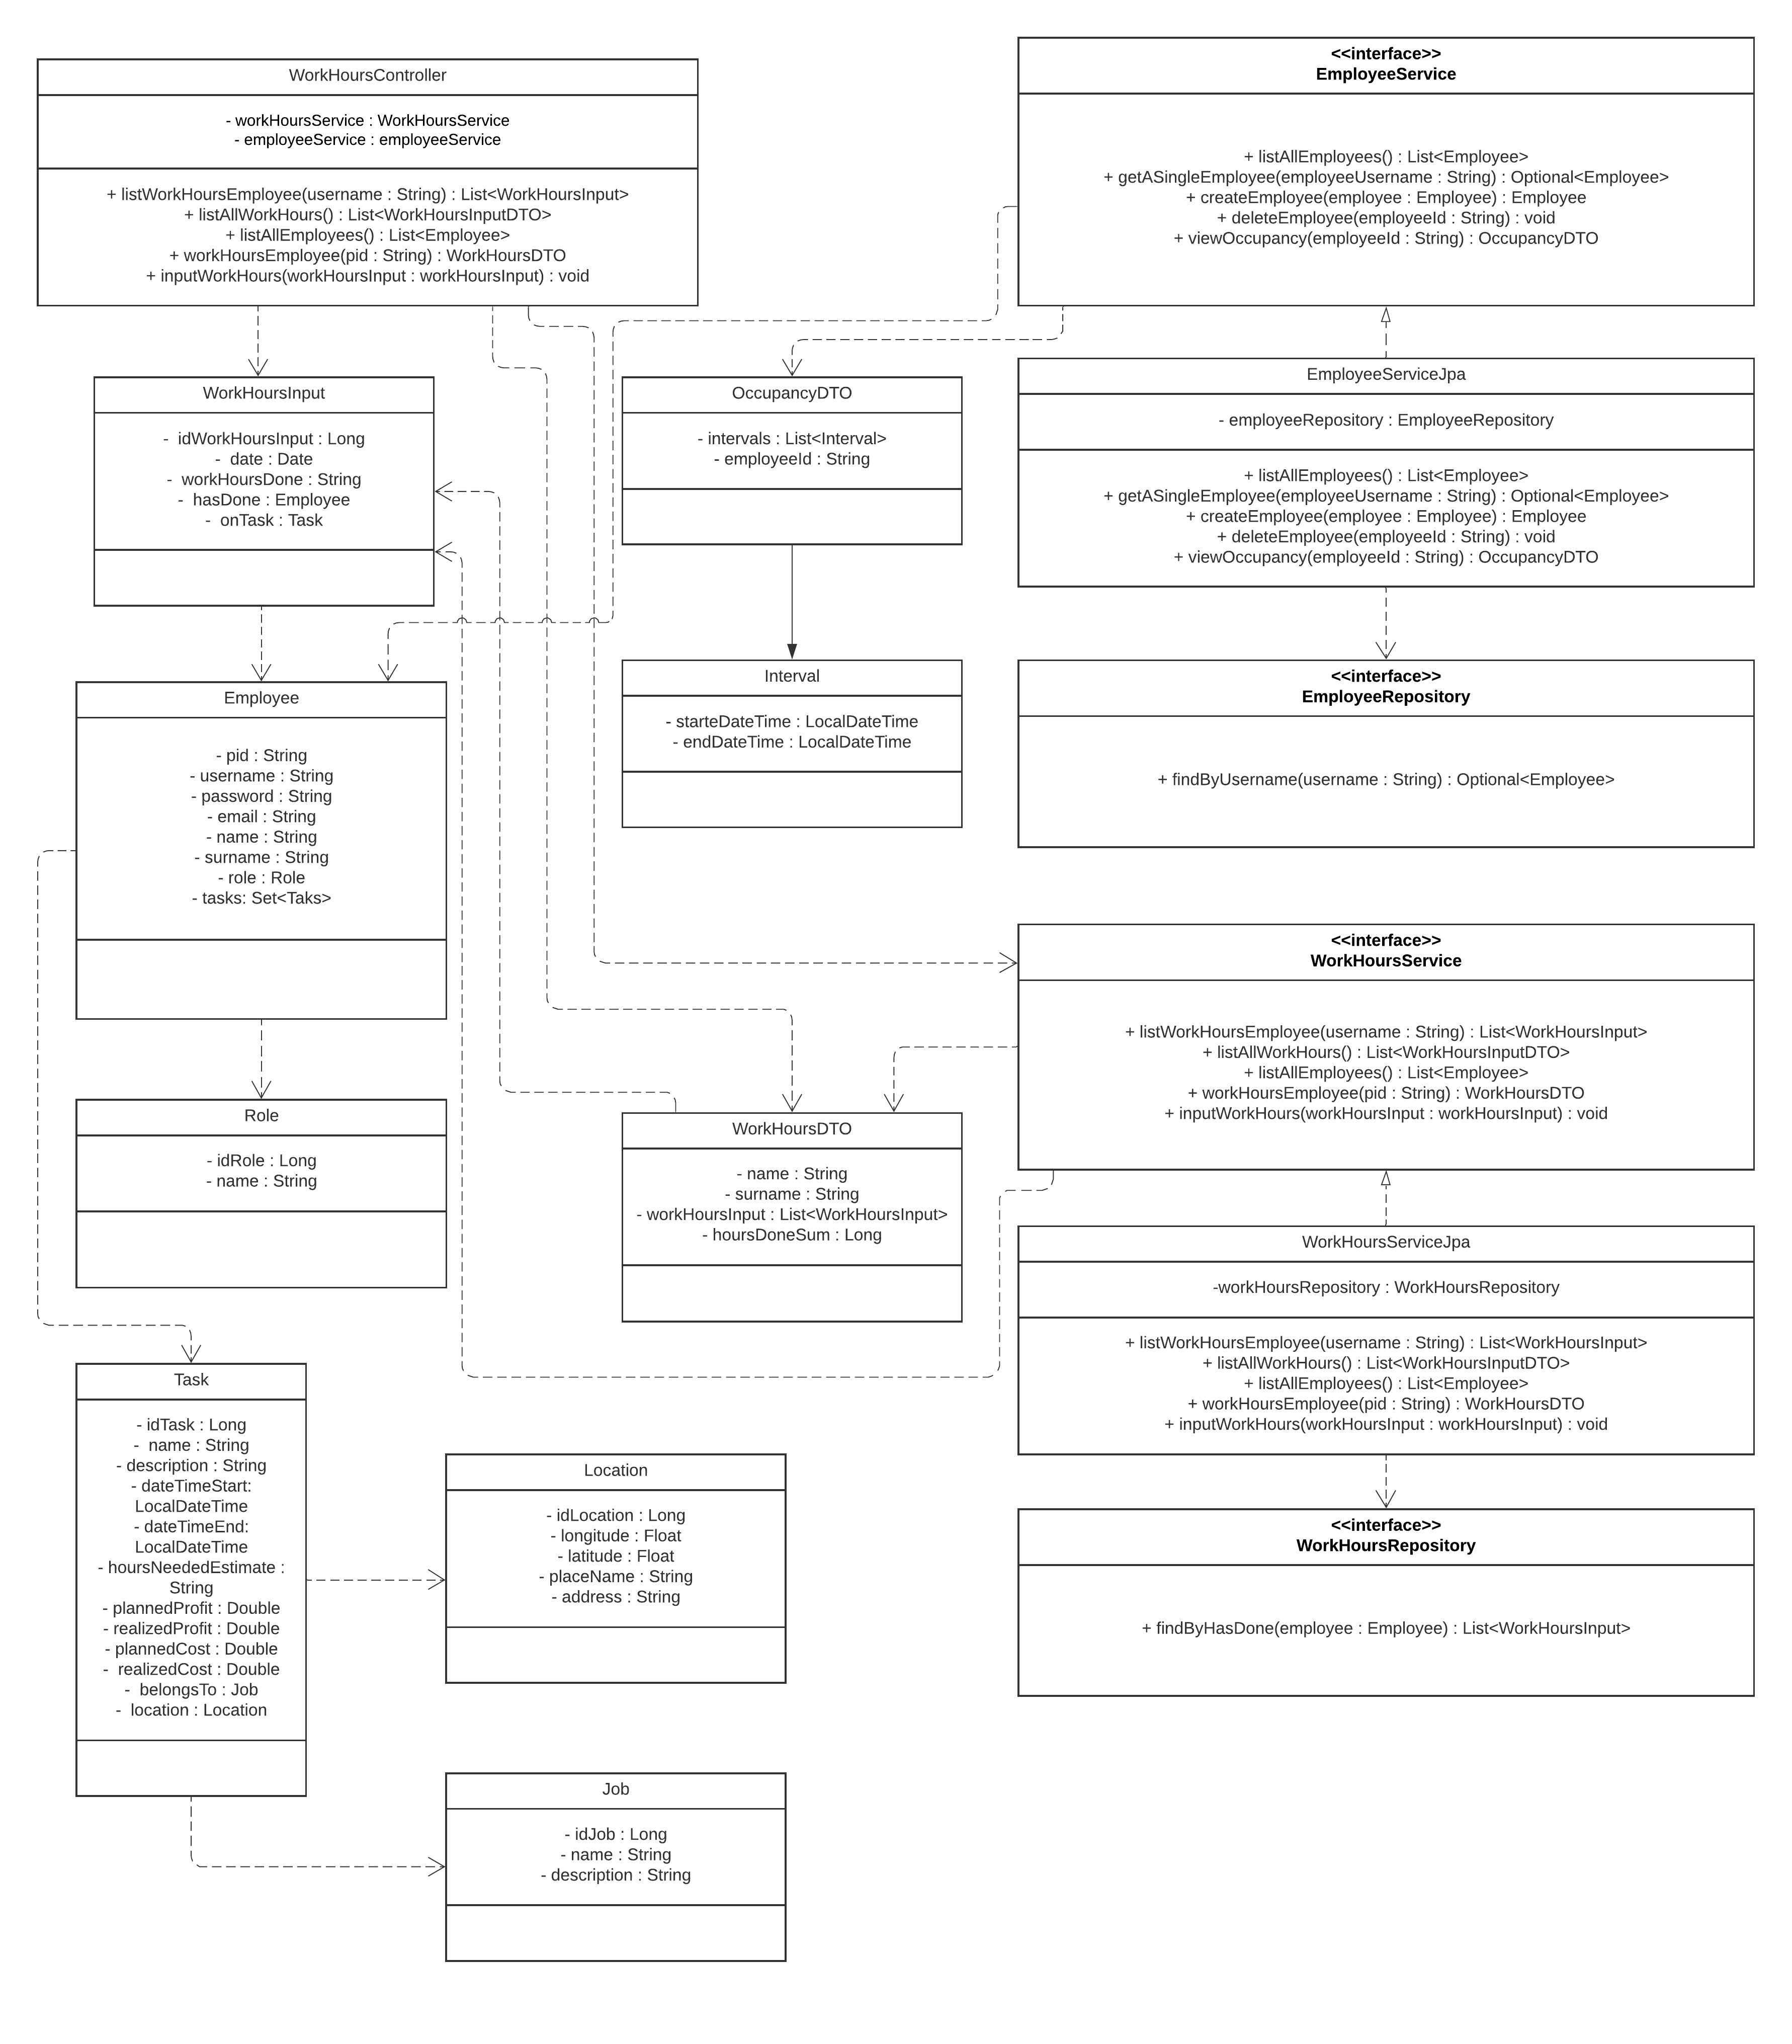
\includegraphics[width=\textwidth]{slike/Dijagram razreda - WorkHoursController.jpg}
					\caption{Dijagram razreda WorkHoursController}
				\end{figure}
			
			
			\eject
			\begin{figure}[H]
					\centering
					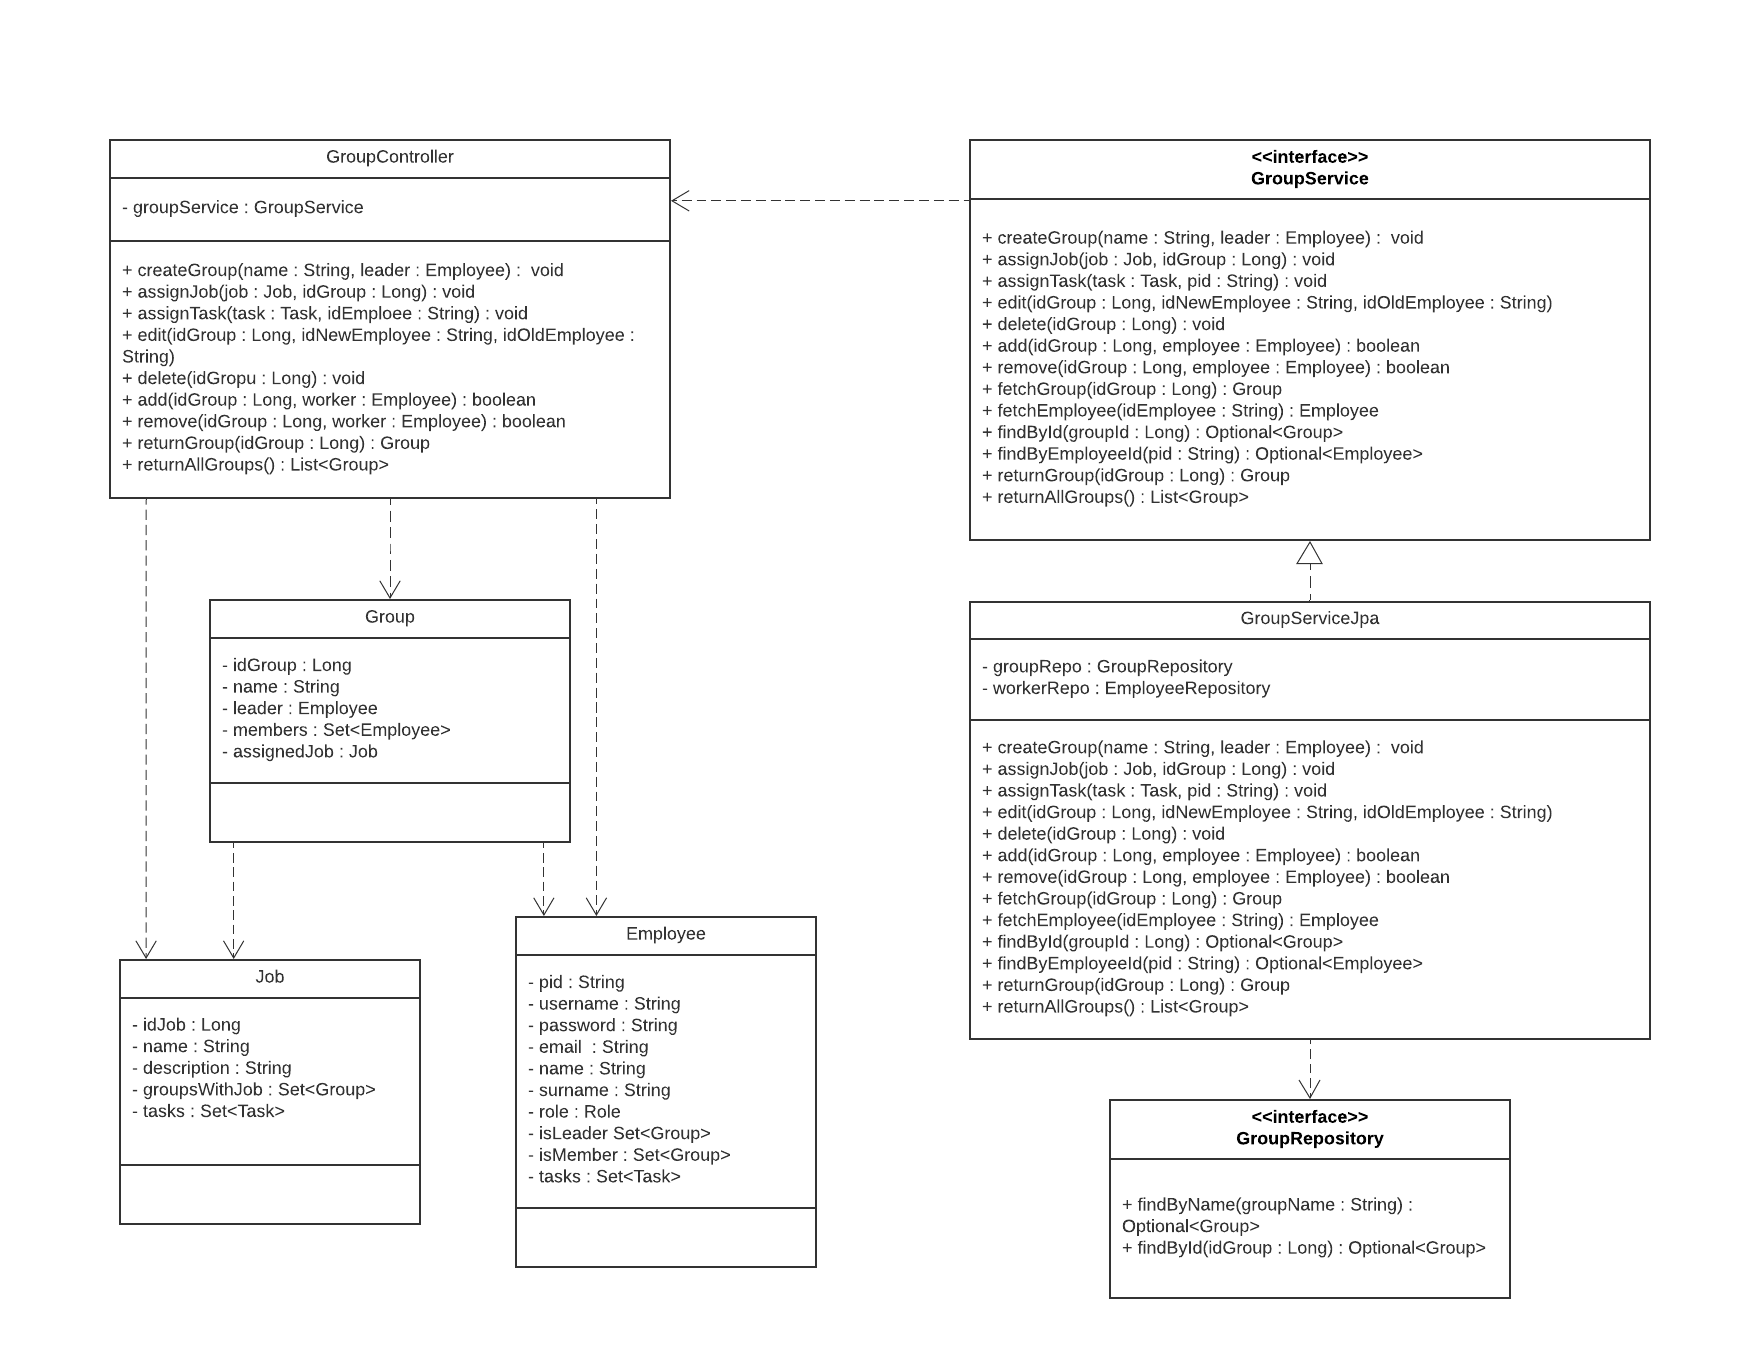
\includegraphics[width=\textwidth]{slike/UML class - GroupController.png}
					\caption{Dijagram razreda GroupController}
				\end{figure}
			
			
			\eject
			\begin{figure}[H]
					\centering
					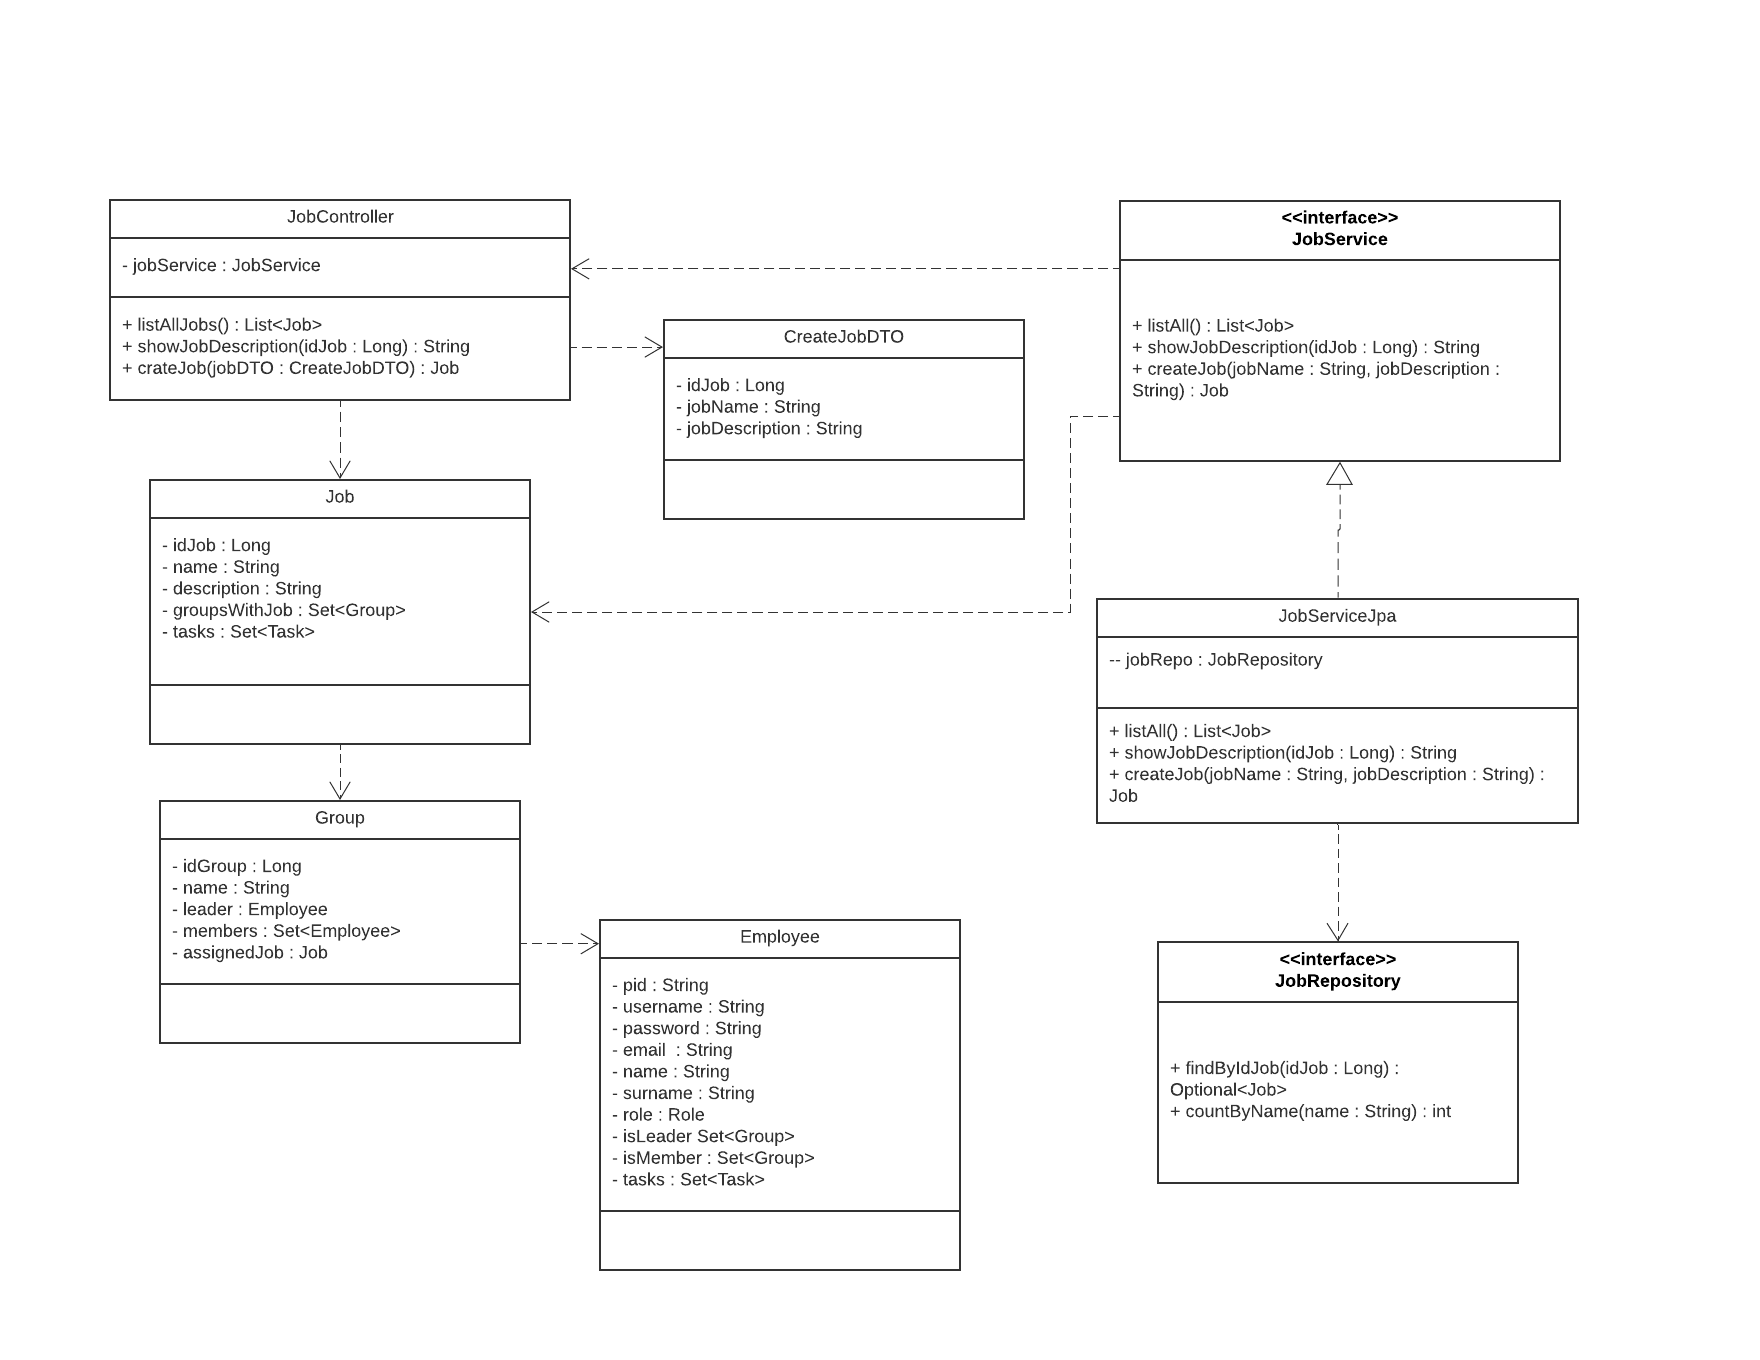
\includegraphics[width=\textwidth]{slike/UML class - JobController.png}
					\caption{Dijagram razreda JobController}
				\end{figure}
			
			
			\eject
			\begin{figure}[H]
					\centering
					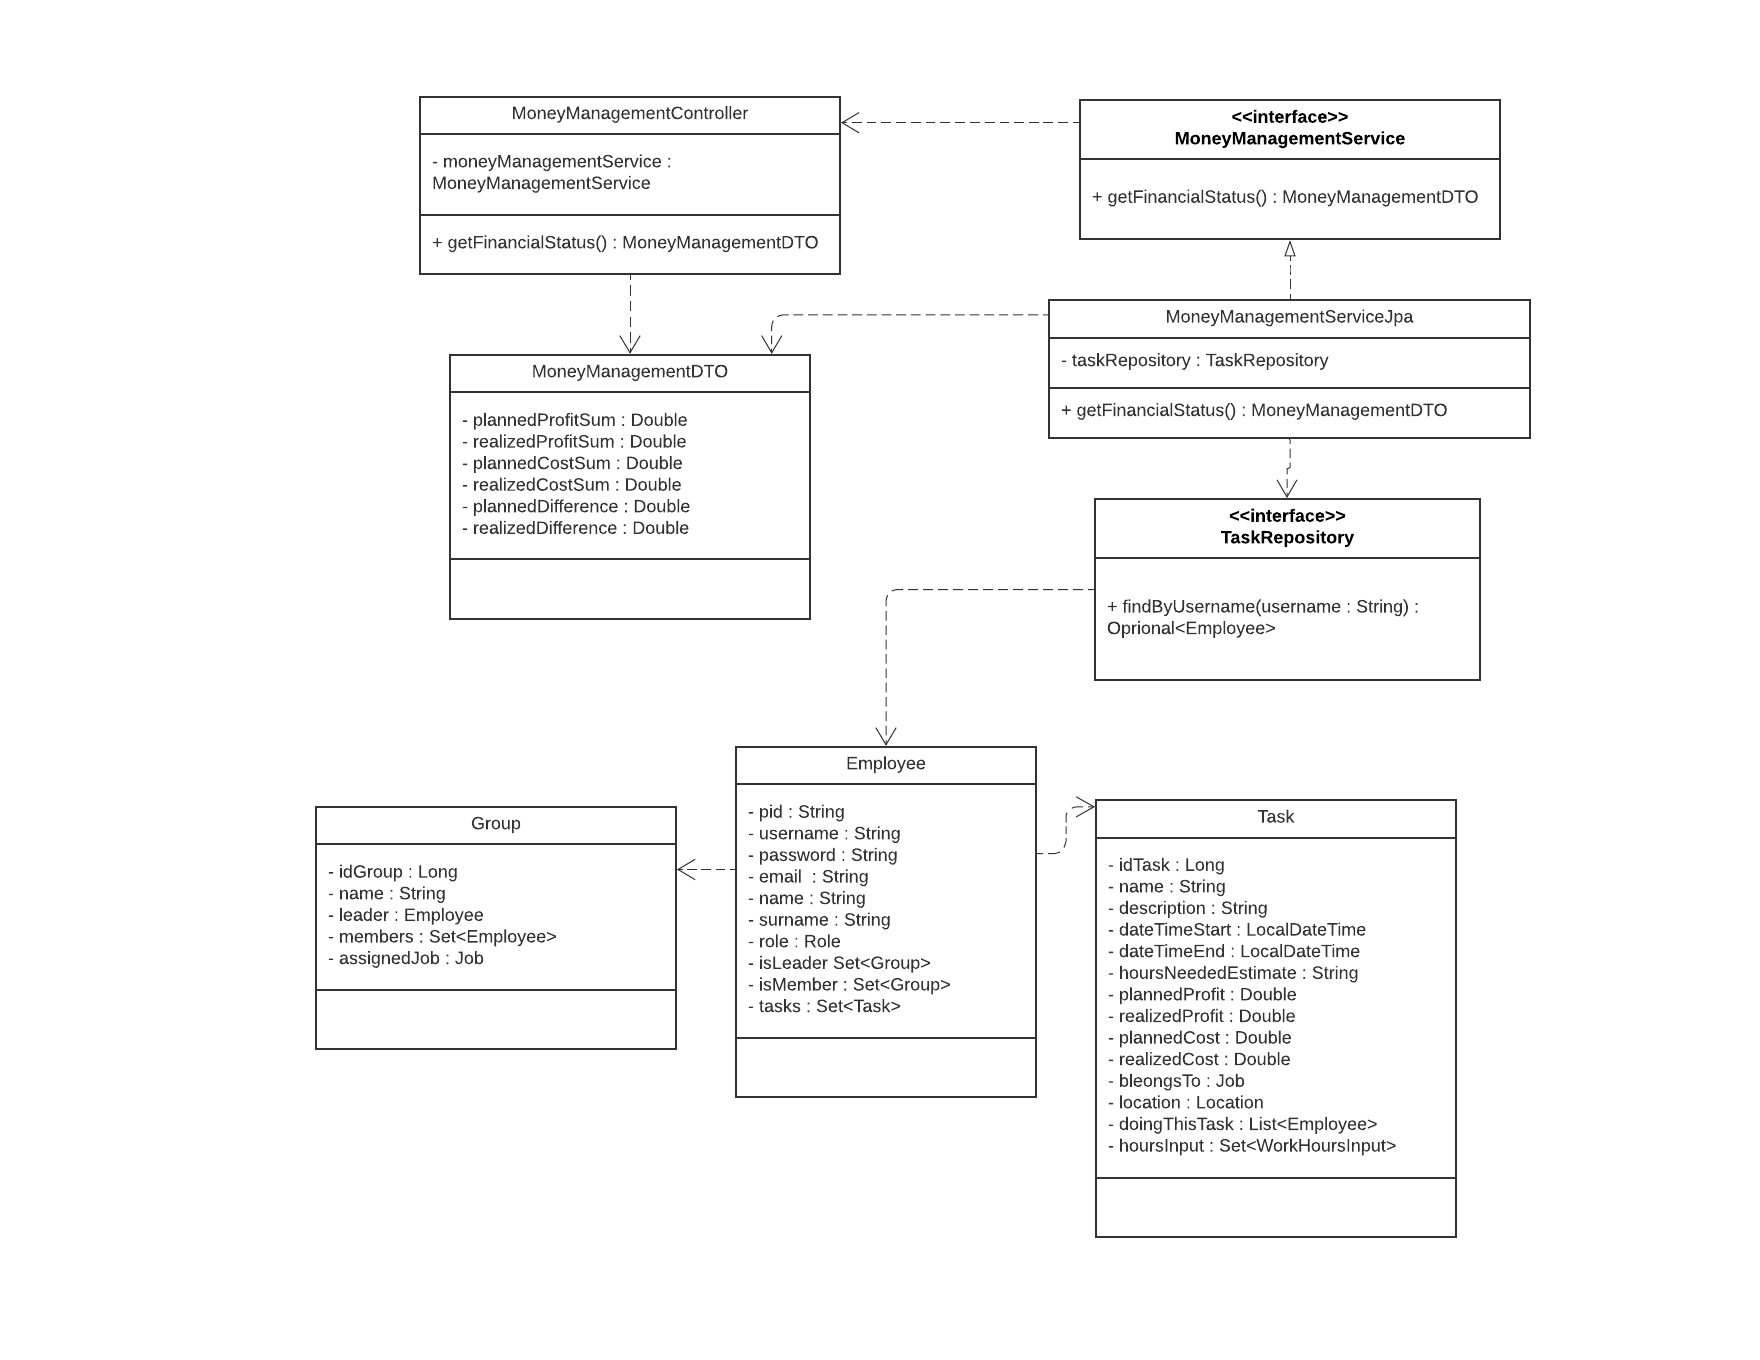
\includegraphics[width=\textwidth]{slike/UML class - MoneyManagementController.png}
					\caption{Dijagram razreda MoneyManagementController}
				\end{figure}
			
			
			\eject
			\begin{figure}[H]
					\centering
					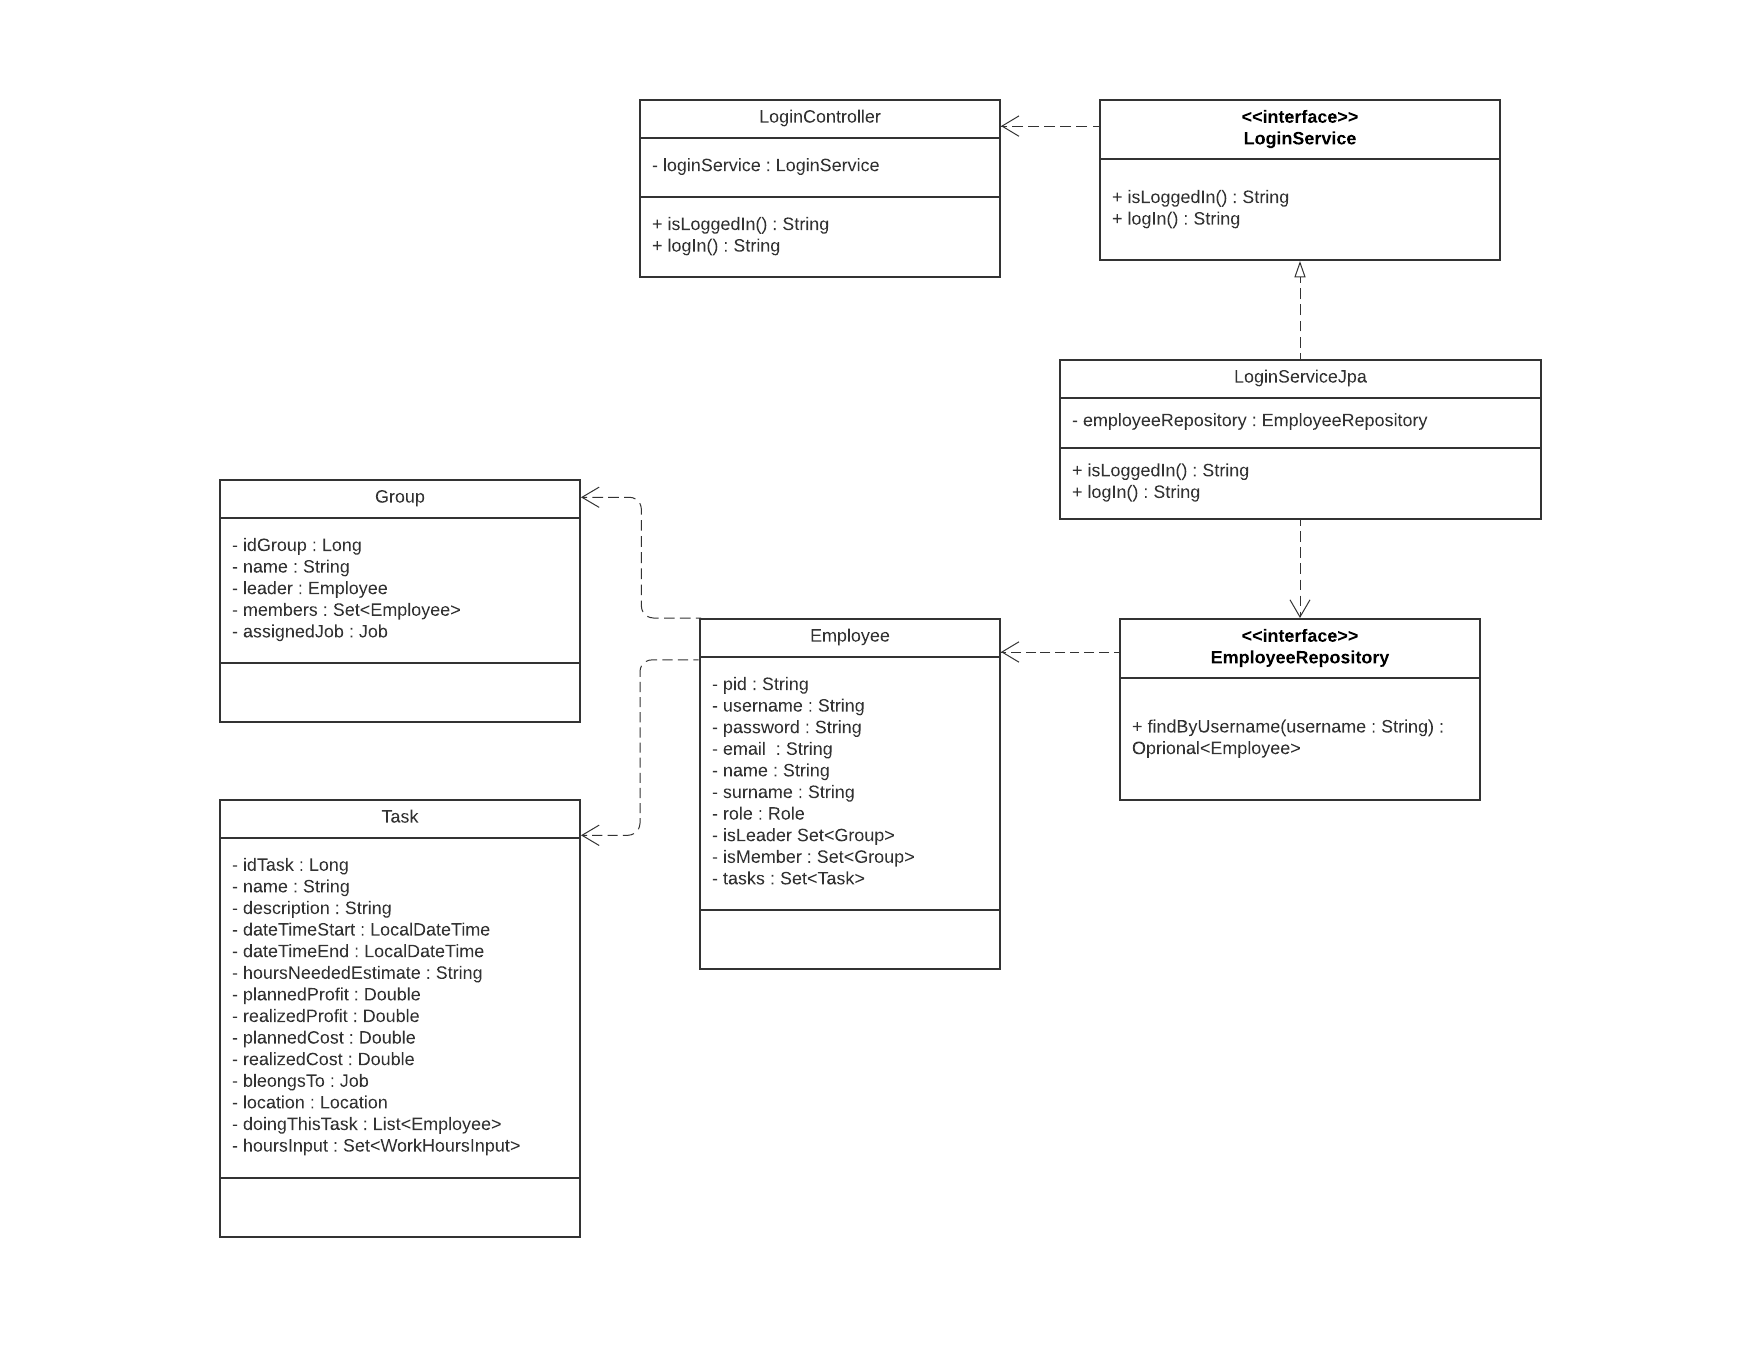
\includegraphics[width=\textwidth]{slike/UML class - LoginController.png}
					\caption{Dijagram razreda LoginController}
				\end{figure}
			
			
			\eject
			
		
		\section{Dijagram stanja}
			
			
			\textbf{\textit{dio 2. revizije}}\\
			
			\textit{Potrebno je priložiti dijagram stanja i opisati ga. Dovoljan je jedan dijagram stanja koji prikazuje \textbf{značajan dio funkcionalnosti} sustava. Na primjer, stanja korisničkog sučelja i tijek korištenja neke ključne funkcionalnosti jesu značajan dio sustava, a registracija i prijava nisu. }
			
			
			\eject 
		
		\section{Dijagram aktivnosti}
			
			\textbf{\textit{dio 2. revizije}}\\
			
			 \textit{Potrebno je priložiti dijagram aktivnosti s pripadajućim opisom. Dijagram aktivnosti treba prikazivati značajan dio sustava.}
			
			\eject
		\section{Dijagram komponenti}
		
			\textbf{\textit{dio 2. revizije}}\\
		
			 \textit{Potrebno je priložiti dijagram komponenti s pripadajućim opisom. Dijagram komponenti treba prikazivati strukturu cijele aplikacije.}